% This file was converted to LaTeX by Writer2LaTeX ver. 1.4
% see http://writer2latex.sourceforge.net for more info
\documentclass[12pt]{article}
\usepackage[utf8]{inputenc}
\usepackage[T1]{fontenc}
\usepackage[english]{babel}
\usepackage{amsmath}
\usepackage{amssymb,amsfonts,textcomp}
\usepackage{array}
\usepackage{hhline}
\usepackage{hyperref}
\hypersetup{colorlinks=true, linkcolor=blue, citecolor=blue, filecolor=blue, urlcolor=blue}
\usepackage{graphicx}
% footnotes configuration
\makeatletter
\renewcommand\thefootnote{\arabic{footnote}}
\makeatother
\newcommand\textsubscript[1]{\ensuremath{{}_{\text{#1}}}}
% Text styles
\newcommand\textstyleFootnoteSymbol[1]{{\fontsize{6.5pt}{7.8pt}\selectfont #1}}
% Headings and outline numbering
\makeatletter
\renewcommand\subsection{\@startsection{subsection}{2}{0.0cm}{0.222in}{0.0835in}{\normalfont\normalsize\fontsize{16pt}{19.2pt}\selectfont\rmfamily\bfseries\raggedright}}
\renewcommand\@seccntformat[1]{\csname @textstyle#1\endcsname{\csname the#1\endcsname}\csname @distance#1\endcsname}
\setcounter{secnumdepth}{0}
\newcommand\@distancesection{}
\newcommand\@textstylesection[1]{#1}
\newcommand\@distancesubsection{}
\newcommand\@textstylesubsection[1]{#1}
\makeatother
\raggedbottom
% Paragraph styles
\renewcommand\familydefault{\rmdefault}
\newenvironment{styleStandard}{\renewcommand\baselinestretch{1.0}\setlength\leftskip{0cm}\setlength\rightskip{0cm plus 1fil}\setlength\parindent{0cm}\setlength\parfillskip{0pt plus 1fil}\setlength\parskip{0in plus 1pt}\writerlistparindent\writerlistleftskip\leavevmode\normalfont\normalsize\writerlistlabel\ignorespaces}{\unskip\vspace{0in plus 1pt}\par}
\newenvironment{stylelsAbstract}{\renewcommand\baselinestretch{1.0}\setlength\leftskip{0.5in}\setlength\rightskip{0.5in}\setlength\parindent{0in}\setlength\parfillskip{0pt plus 1fil}\setlength\parskip{0in plus 1pt}\writerlistparindent\writerlistleftskip\leavevmode\normalfont\normalsize\itshape\writerlistlabel\ignorespaces}{\unskip\vspace{0in plus 1pt}\par}
\newenvironment{stylelsSectioni}{\renewcommand\baselinestretch{1.0}\setlength\leftskip{0.248in}\setlength\rightskip{0in plus 1fil}\setlength\parindent{-0.248in}\setlength\parfillskip{0pt plus 1fil}\setlength\parskip{0in plus 1pt}\writerlistparindent\writerlistleftskip\leavevmode\normalfont\normalsize\fontsize{18pt}{21.6pt}\selectfont\bfseries\writerlistlabel\ignorespaces}{\unskip\vspace{0in plus 1pt}\par}
\newenvironment{styleListParagraph}{\renewcommand\baselinestretch{1.0}\setlength\leftskip{0.5in}\setlength\rightskip{0in plus 1fil}\setlength\parindent{0in}\setlength\parfillskip{0pt plus 1fil}\setlength\parskip{0in plus 1pt}\writerlistparindent\writerlistleftskip\leavevmode\normalfont\normalsize\writerlistlabel\ignorespaces}{\unskip\vspace{0in plus 1pt}\par}
\newenvironment{styleNormalWeb}{\renewcommand\baselinestretch{1.0}\setlength\leftskip{0cm}\setlength\rightskip{0cm plus 1fil}\setlength\parindent{0cm}\setlength\parfillskip{0pt plus 1fil}\setlength\parskip{0.1945in plus 0.01945in}\writerlistparindent\writerlistleftskip\leavevmode\normalfont\normalsize\writerlistlabel\ignorespaces}{\unskip\vspace{0.1945in plus 0.01945in}\par}
\newenvironment{styleDefault}{\renewcommand\baselinestretch{1.0}\setlength\leftskip{0cm}\setlength\rightskip{0cm plus 1fil}\setlength\parindent{0cm}\setlength\parfillskip{0pt plus 1fil}\setlength\parskip{0in plus 1pt}\writerlistparindent\writerlistleftskip\leavevmode\normalfont\normalsize\writerlistlabel\ignorespaces}{\unskip\vspace{0in plus 1pt}\par}
% List styles
\newcommand\writerlistleftskip{}
\newcommand\writerlistparindent{}
\newcommand\writerlistlabel{}
\newcommand\writerlistremovelabel{\aftergroup\let\aftergroup\writerlistparindent\aftergroup\relax\aftergroup\let\aftergroup\writerlistlabel\aftergroup\relax}
\newcounter{listWWNumxxiileveli}
\newcounter{listWWNumxxiilevelii}[listWWNumxxiileveli]
\newcounter{listWWNumxxiileveliii}[listWWNumxxiilevelii]
\newcounter{listWWNumxxiileveliv}[listWWNumxxiileveliii]
\renewcommand\thelistWWNumxxiileveli{\arabic{listWWNumxxiileveli}}
\renewcommand\thelistWWNumxxiilevelii{\arabic{listWWNumxxiileveli}.\arabic{listWWNumxxiilevelii}}
\renewcommand\thelistWWNumxxiileveliii{\arabic{listWWNumxxiileveli}.\arabic{listWWNumxxiilevelii}.\arabic{listWWNumxxiileveliii}}
\renewcommand\thelistWWNumxxiileveliv{\arabic{listWWNumxxiileveli}.\arabic{listWWNumxxiilevelii}.\arabic{listWWNumxxiileveliii}.\arabic{listWWNumxxiileveliv}}
\newcommand\labellistWWNumxxiileveli{\thelistWWNumxxiileveli.}
\newcommand\labellistWWNumxxiilevelii{\thelistWWNumxxiilevelii.}
\newcommand\labellistWWNumxxiileveliii{\thelistWWNumxxiileveliii.}
\newcommand\labellistWWNumxxiileveliv{\thelistWWNumxxiileveliv.}
\newenvironment{listWWNumxxiileveli}{\def\writerlistleftskip{\setlength\leftskip{0.5in}}\def\writerlistparindent{}\def\writerlistlabel{}\def\item{\def\writerlistparindent{\setlength\parindent{-0.25in}}\def\writerlistlabel{\stepcounter{listWWNumxxiileveli}\makebox[0cm][l]{\labellistWWNumxxiileveli}\hspace{-0.635cm}\writerlistremovelabel}}}{}
\newenvironment{listWWNumxxiilevelii}{\def\writerlistleftskip{\setlength\leftskip{1in}}\def\writerlistparindent{}\def\writerlistlabel{}\def\item{\def\writerlistparindent{\setlength\parindent{-0.25in}}\def\writerlistlabel{\stepcounter{listWWNumxxiilevelii}\makebox[0cm][l]{\labellistWWNumxxiilevelii}\hspace{-1.905cm}\writerlistremovelabel}}}{}
\newenvironment{listWWNumxxiileveliii}{\def\writerlistleftskip{\setlength\leftskip{1.5in}}\def\writerlistparindent{}\def\writerlistlabel{}\def\item{\def\writerlistparindent{\setlength\parindent{-0.1252in}}\def\writerlistlabel{\stepcounter{listWWNumxxiileveliii}\makebox[0cm][r]{\labellistWWNumxxiileveliii}\hspace{-3.4919918cm}\writerlistremovelabel}}}{}
\newenvironment{listWWNumxxiileveliv}{\def\writerlistleftskip{\setlength\leftskip{2in}}\def\writerlistparindent{}\def\writerlistlabel{}\def\item{\def\writerlistparindent{\setlength\parindent{-0.25in}}\def\writerlistlabel{\stepcounter{listWWNumxxiileveliv}\makebox[0cm][l]{\labellistWWNumxxiileveliv}\hspace{-4.4449997cm}\writerlistremovelabel}}}{}
\newcounter{listWWNumxxivleveli}
\newcounter{listWWNumxxivlevelii}[listWWNumxxivleveli]
\newcounter{listWWNumxxivleveliii}[listWWNumxxivlevelii]
\newcounter{listWWNumxxivleveliv}[listWWNumxxivleveliii]
\renewcommand\thelistWWNumxxivleveli{\arabic{listWWNumxxivleveli}}
\renewcommand\thelistWWNumxxivlevelii{\arabic{listWWNumxxivleveli}.\arabic{listWWNumxxivlevelii}}
\renewcommand\thelistWWNumxxivleveliii{\arabic{listWWNumxxivleveli}.\arabic{listWWNumxxivlevelii}.\arabic{listWWNumxxivleveliii}}
\renewcommand\thelistWWNumxxivleveliv{\arabic{listWWNumxxivleveli}.\arabic{listWWNumxxivlevelii}.\arabic{listWWNumxxivleveliii}.\arabic{listWWNumxxivleveliv}}
\newcommand\labellistWWNumxxivleveli{\thelistWWNumxxivleveli.}
\newcommand\labellistWWNumxxivlevelii{\thelistWWNumxxivlevelii.}
\newcommand\labellistWWNumxxivleveliii{\thelistWWNumxxivleveliii.}
\newcommand\labellistWWNumxxivleveliv{\thelistWWNumxxivleveliv.}
\newenvironment{listWWNumxxivleveli}{\def\writerlistleftskip{\setlength\leftskip{0.5in}}\def\writerlistparindent{}\def\writerlistlabel{}\def\item{\def\writerlistparindent{\setlength\parindent{-0.25in}}\def\writerlistlabel{\stepcounter{listWWNumxxivleveli}\makebox[0cm][l]{\labellistWWNumxxivleveli}\hspace{-0.635cm}\writerlistremovelabel}}}{}
\newenvironment{listWWNumxxivlevelii}{\def\writerlistleftskip{\setlength\leftskip{1in}}\def\writerlistparindent{}\def\writerlistlabel{}\def\item{\def\writerlistparindent{\setlength\parindent{-0.25in}}\def\writerlistlabel{\stepcounter{listWWNumxxivlevelii}\makebox[0cm][l]{\labellistWWNumxxivlevelii}\hspace{-1.905cm}\writerlistremovelabel}}}{}
\newenvironment{listWWNumxxivleveliii}{\def\writerlistleftskip{\setlength\leftskip{1.5in}}\def\writerlistparindent{}\def\writerlistlabel{}\def\item{\def\writerlistparindent{\setlength\parindent{-0.1252in}}\def\writerlistlabel{\stepcounter{listWWNumxxivleveliii}\makebox[0cm][r]{\labellistWWNumxxivleveliii}\hspace{-3.4919918cm}\writerlistremovelabel}}}{}
\newenvironment{listWWNumxxivleveliv}{\def\writerlistleftskip{\setlength\leftskip{2in}}\def\writerlistparindent{}\def\writerlistlabel{}\def\item{\def\writerlistparindent{\setlength\parindent{-0.25in}}\def\writerlistlabel{\stepcounter{listWWNumxxivleveliv}\makebox[0cm][l]{\labellistWWNumxxivleveliv}\hspace{-4.4449997cm}\writerlistremovelabel}}}{}
\newcounter{listWWNumxxvleveli}
\newcounter{listWWNumxxvlevelii}[listWWNumxxvleveli]
\newcounter{listWWNumxxvleveliii}[listWWNumxxvlevelii]
\newcounter{listWWNumxxvleveliv}[listWWNumxxvleveliii]
\renewcommand\thelistWWNumxxvleveli{\roman{listWWNumxxvleveli}}
\renewcommand\thelistWWNumxxvlevelii{\alph{listWWNumxxvlevelii}}
\renewcommand\thelistWWNumxxvleveliii{\roman{listWWNumxxvleveliii}}
\renewcommand\thelistWWNumxxvleveliv{\arabic{listWWNumxxvleveliv}}
\newcommand\labellistWWNumxxvleveli{(\thelistWWNumxxvleveli)}
\newcommand\labellistWWNumxxvlevelii{\thelistWWNumxxvlevelii.}
\newcommand\labellistWWNumxxvleveliii{\thelistWWNumxxvleveliii.}
\newcommand\labellistWWNumxxvleveliv{\thelistWWNumxxvleveliv.}
\newenvironment{listWWNumxxvleveli}{\def\writerlistleftskip{\setlength\leftskip{0.75in}}\def\writerlistparindent{}\def\writerlistlabel{}\def\item{\def\writerlistparindent{\setlength\parindent{-0.5in}}\def\writerlistlabel{\stepcounter{listWWNumxxvleveli}\makebox[0cm][l]{\labellistWWNumxxvleveli}\hspace{-0.635cm}\writerlistremovelabel}}}{}
\newenvironment{listWWNumxxvlevelii}{\def\writerlistleftskip{\setlength\leftskip{1in}}\def\writerlistparindent{}\def\writerlistlabel{}\def\item{\def\writerlistparindent{\setlength\parindent{-0.25in}}\def\writerlistlabel{\stepcounter{listWWNumxxvlevelii}\makebox[0cm][l]{\labellistWWNumxxvlevelii}\hspace{-1.905cm}\writerlistremovelabel}}}{}
\newenvironment{listWWNumxxvleveliii}{\def\writerlistleftskip{\setlength\leftskip{1.5in}}\def\writerlistparindent{}\def\writerlistlabel{}\def\item{\def\writerlistparindent{\setlength\parindent{-0.1252in}}\def\writerlistlabel{\stepcounter{listWWNumxxvleveliii}\makebox[0cm][r]{\labellistWWNumxxvleveliii}\hspace{-3.4919918cm}\writerlistremovelabel}}}{}
\newenvironment{listWWNumxxvleveliv}{\def\writerlistleftskip{\setlength\leftskip{2in}}\def\writerlistparindent{}\def\writerlistlabel{}\def\item{\def\writerlistparindent{\setlength\parindent{-0.25in}}\def\writerlistlabel{\stepcounter{listWWNumxxvleveliv}\makebox[0cm][l]{\labellistWWNumxxvleveliv}\hspace{-4.4449997cm}\writerlistremovelabel}}}{}
\newcounter{qwerty}
\renewcommand\theqwerty{\arabic{qwerty}}
\title{}
\author{}
\date{2019-07-23}
\begin{document}
\title{\textsuperscript{The }Romance Person Case Constraint is not about clitic clusters }
\maketitle

\begin{styleStandard}
\textbf{Michelle Sheehan}
\end{styleStandard}

\begin{styleStandard}
\textbf{Anglia Ruskin University}
\end{styleStandard}

\begin{stylelsAbstract}
\textbf{Abstract.} This paper provides further evidence that the Person Case Constraint (PCC) in Romance is not limited to clitic clusters. Previously, this has been shown only for Spanish (Ormazabal and Romero 2013), but I show that, in Italian, French, and Catalan causatives, a 1\textsuperscript{st}/2\textsuperscript{nd} person direct object is incompatible not only with dative clitics but also with full dative arguments (see also Postal 1989, Bonet 1991). This is different from the manifestation of the PCC in ditransitive contexts where only dative clitics are ruled out. The difference follows, I argue, if ditransitives in these languages have two underlying structures so that a DP introduced by ‘a/à’ can be either dative or locative, in line with broader cross-linguistic patterns (see Harley 2002; Demonte 1995, Cuervo 2003 on Spanish; Anagnostopoulou 2003, Fournier 2010 on French; Holmberg, Sheehan \& van der Wal 2018 on Italian, and the discussion in the introduction to this volume). For this reason, indirect object DPs marked with a/à must trigger PCC effects in causatives but not in ditransitives, as only in the former are they unambiguously dative. Further support for this claim comes from Spanish, a language which morphologically distinguishes locative vs. dative phrases in ditransitives via clitic doubling (Cuervo 2003) and which shows PCC effects with all animate direct objects (Ormazabal and Romero 2007, 2013). I show that these facts are compatible with approaches to the PCC based on intervention (Anagnostopoulou 2003, 2005 amongst others), but raise challenges for those which rely crucially on the weak/clitic status of datives (Bianchi 2006, Stegovec 2017). 
\end{stylelsAbstract}

\begin{stylelsSectioni}
1. The Person Case Constraint
\end{stylelsSectioni}

\begin{styleStandard}
Like many languages, French, Spanish, Catalan and Italian are subject to the Person Case Constraint (PCC), originally called the \textit{*me lui constraint} by Perlmutter (1971): \footnote{ Though the PCC was first discovered as the \textit{*me-lui constraint} and investigated in Romance (Perlmutter 1971), it has been found to hold in a wide range of unrelated languages (see Bonet 1991, Albizu 1997, Rezac 2008, Haspelmath 2004, Adger and Harbour 2007). In fact, one of the key contributions of Bonet (1991) was to unify the Romance constraint with a parallel effect observed in rich agreement systems. I thank an anonymous reviewer for asking me to clarify this. See also Bonet (2007) for an overview. }
\end{styleStandard}

\begin{styleStandard}
(\stepcounter{qwerty}{\theqwerty})\ \ Strong Person Case Constraint (based on Bonet 1991: 181-182)
\end{styleStandard}


\setcounter{listWWNumxxiileveli}{0}
\begin{listWWNumxxiileveli}
\item 

\setcounter{listWWNumxxiilevelii}{0}
\begin{listWWNumxxiilevelii}
\item 

\setcounter{listWWNumxxiileveliii}{0}
\begin{listWWNumxxiileveliii}
\item 

\setcounter{listWWNumxxiileveliv}{0}
\begin{listWWNumxxiileveliv}
\item 
\begin{styleListParagraph}
In a combination of a direct object and an indirect object, the direct object has to be third person.
\end{styleListParagraph}
\begin{styleListParagraph}
If both the indirect object and the direct object are phonologically weak. 
\end{styleListParagraph}
\end{listWWNumxxiileveliv}
\end{listWWNumxxiileveliii}
\end{listWWNumxxiilevelii}
\end{listWWNumxxiileveli}
\begin{styleStandard}
In Romance languages, this strong version of the constraint rules out the possibility of a 1\textsuperscript{st}/2\textsuperscript{nd} person direct object clitic (glossed here as \textsc{acc}) in the presence of a dative clitic, for example, the following combination of 1\textsuperscript{st} person accusative and 3\textsuperscript{rd} person dative clitics (see Perlmutter 1971, Kayne 1975, Postal 1981 on the PCC in French):
\end{styleStandard}

\begin{styleStandard}
(\stepcounter{qwerty}{\theqwerty})\ \ French (Kayne 1975: 173)
\end{styleStandard}

\begin{styleStandard}
\ \ *Paul \ \ me \ \ \ \ \ \ lui \ \ \ \ \ \ présentera.
\end{styleStandard}

\begin{styleStandard}
\ \ she \ \ me.\textsc{acc}= \ \ him.\textsc{dat=} present.\textsc{3sg.fut}
\end{styleStandard}

\begin{styleStandard}
\ \ Intended: ‘Paul will introduce me to him.’
\end{styleStandard}

\begin{styleStandard}
The presence of (1b) is seemingly crucial to the definition of the PCC because the effect disappears, in ditransitives, where the indirect object is a non-clitic (Kayne 1975, Rezac 2008). The meaning intended to be conveyed by (2) can easily be conveyed using an unfocussed tonic pronoun introduced by à, which is exceptionally allowed in such contexts:\footnote{ I gloss \textit{a/à} as ‘to’ throughout for expositional purposes, but one of the main claims of this paper is that sometime this morpheme is a realisation of dative case marking and at other times it is a locative preposition. }
\end{styleStandard}

\begin{styleStandard}
(\stepcounter{qwerty}{\theqwerty})\ \ French (Kayne 1975: 174)\ \ 
\end{styleStandard}

\begin{styleStandard}
Paul \ \ me \ \ \ \ présentera \ \ \ \ à \ \ lui.
\end{styleStandard}

\begin{styleStandard}
\ \ Paul\ \ me.\textsc{acc}=\ \ present.\textsc{3s.fut} \ \ to \ \ him
\end{styleStandard}

\begin{styleStandard}
\ \ ‘Paul will introduce me to him.’
\end{styleStandard}

\begin{styleStandard}
At least for some speakers, Italian, Spanish and Catalan seem to be subject to a weaker form of the PCC, as described by Bonet (1991), again building on Perlmutter (1971):\textstyleFootnoteSymbol{ }\footnote{ There are other subtle differences between the languages too, which require an explanation, notably order in the clitic cluster. A more substantive difference is that Italian, like Spanish and Catalan and unlike French, allows 1st/2nd person reflexive direct objects to combine with dative clitics (see Kayne 1975, Bianchi 2006). We abstract away from this difference here for reasons of space.}
\end{styleStandard}

\begin{styleStandard}
(\stepcounter{qwerty}{\theqwerty})\ \ Weak Person Case Constraint (based on Bonet 1991: 181-182): \ 
\end{styleStandard}


\setcounter{listWWNumxxivleveli}{0}
\begin{listWWNumxxivleveli}
\item 

\setcounter{listWWNumxxivlevelii}{0}
\begin{listWWNumxxivlevelii}
\item 

\setcounter{listWWNumxxivleveliii}{0}
\begin{listWWNumxxivleveliii}
\item 

\setcounter{listWWNumxxivleveliv}{0}
\begin{listWWNumxxivleveliv}
\item 
\begin{styleListParagraph}
In a combination of a direct object and an indirect object, if there is a third person, it has to be the direct object.
\end{styleListParagraph}
\end{listWWNumxxivleveliv}
\end{listWWNumxxivleveliii}
\end{listWWNumxxivlevelii}
\end{listWWNumxxivleveli}

\setcounter{listWWNumxxiileveli}{0}
\begin{listWWNumxxiileveli}
\item 

\setcounter{listWWNumxxiilevelii}{0}
\begin{listWWNumxxiilevelii}
\item 

\setcounter{listWWNumxxiileveliii}{0}
\begin{listWWNumxxiileveliii}
\item 

\setcounter{listWWNumxxiileveliv}{0}
\begin{listWWNumxxiileveliv}
\item 
\begin{styleListParagraph}
If both the indirect object and the direct object are phonologically weak. 
\end{styleListParagraph}
\end{listWWNumxxiileveliv}
\end{listWWNumxxiileveliii}
\end{listWWNumxxiilevelii}
\end{listWWNumxxiileveli}
\begin{styleStandard}
In the Romance context, this weaker version of the PCC allows for the possibility of a 1\textsuperscript{st}/2\textsuperscript{nd} person accusative clitic as long as the dative is also 1\textsuperscript{st}/2\textsuperscript{nd} person, with many speakers preferring a reading whereby the 2\textsuperscript{nd} person clitic functions as the direct object in such cases (see Bonet 1991: 180, fn 5 citing a personal communication from Alex Alsina on Catalan; Ormazabal and Romero 2010: 332 on Spanish, but see also the discussion in Bonet 2007):
\end{styleStandard}

\begin{styleStandard}
(\stepcounter{qwerty}{\theqwerty})\ \ Italian (Bianchi 2006: 2027)\textstyleFootnoteSymbol{ }\footnote{ Note that Bianchi actually gives this example to be ungrammatical but then discusses at length the fact that some speakers accept such examples. I represent this with \%.}
\end{styleStandard}

\begin{styleStandard}
\%Mi \ \ ti \ \ \ \ ha \ \ affidato. 
\end{styleStandard}

\begin{styleStandard}
\ \ \textsc{1sg=} \ \ \textsc{2sg=} \ \ has \ \ entrusted
\end{styleStandard}

\begin{styleStandard}
\ \ {}'He entrusted you to me/me to you.’
\end{styleStandard}

\begin{styleStandard}
(\stepcounter{qwerty}{\theqwerty})\ \ Catalan (Bonet 1991: 179)
\end{styleStandard}

\begin{styleStandard}
\%Te’\ \ m \ \ van \ \ recomanar \ \ per \ \ la \ \ feina
\end{styleStandard}

\begin{styleStandard}
\ \ \textsc{2sg=\ \ 1sg} \ \ \textsc{pst} \ \ recommend \ \ for \ \ the \ \ job
\end{styleStandard}

\begin{styleStandard}
‘They recommended me to you/you to me for the job.’
\end{styleStandard}

\begin{styleStandard}
(\stepcounter{qwerty}{\theqwerty})\ \ Spanish (Perlmutter 1971: 61)
\end{styleStandard}

\begin{styleStandard}
\%Te \ \ me \ \ recomendaron \ 
\end{styleStandard}

\begin{styleStandard}
\ \ \textsc{2sg=\ \ 1sg} \ \ recommended.\textsc{3pl}
\end{styleStandard}

\begin{styleStandard}
‘They recommended me to you/you to me.’
\end{styleStandard}

\begin{styleStandard}
French is usually reported to disallow this clitic combination altogether (Kayne 1975, Quicoli 1984) and certainly combinations of 1\textsuperscript{st} and 2\textsuperscript{nd} person objects seem to be more restricted in French than in the other three languages, though Bonet (1991: 180) cites Simpson and Withgott (1986) who report that some speakers nonetheless allow them. 
\end{styleStandard}

\begin{styleStandard}
Ormazabal and Romero (2007) discuss the weak/strong distinction in Romance and note that there is substantial sensitivity to individual verbs and variability across speakers regarding the acceptability of examples like (5)-(7). For this reason, they conclude that there is no clear-cut distinction between strong and weak PCC ‘languages’. In fact, the fact that in combinations of 1\textsuperscript{st} and 2\textsuperscript{nd} person objects, it is almost always the 2\textsuperscript{nd} person clitic which must be the direct object suggests rather that there is merely variation regarding the extent to which person features are decomposed in PCC contexts (see also Anagnostopoulou 2005 for an account along these lines). This can also be seen in Spanish leísta dialects in which 3\textsuperscript{rd} person animate direct objects also trigger PCC effects (Ormazabal and Romero 2007, 2010, 2013):\footnote{ The observant reader will notice that I have not specified that only animate 3\textsuperscript{rd} person singular masculine \textit{clitics} induce PCC effects. Ad we shall see below, this is because animate full DP direct objects marked with personal ‘a’ also trigger PCC effects in Spanish (see Ormazabal and Romero 2013). }
\end{styleStandard}

\begin{styleStandard}
(\stepcounter{qwerty}{\theqwerty})\ \ Spanish (Ormazabal and Romero 2007: 321)
\end{styleStandard}

\begin{styleStandard}
Te \ \ \ \ lo/\ \ \ \ *le \ \ \ \ di \ 
\end{styleStandard}

\begin{styleStandard}
\ \ \textsc{2sg}.\textsc{dat}=\ \ \textsc{3sg.m.acc}/\ \ him.\textsc{acc}=\ \ gave \ 
\end{styleStandard}

\begin{styleStandard}
\ \ ‘I gave it/him to you.’
\end{styleStandard}

\begin{styleStandard}
In these leísta dialects, animate 3\textsuperscript{rd} person singular masculine direct objects are marked with the clitic \textit{le, }rather than \textit{lo,} which is usually reserved for inanimate 3\textsuperscript{rd} person singular masculine direct objects. According to Ormazabal and Romero, the animate direct object clitic \textit{le} is ruled out in (8) in the presence of a dative clitic, as a PCC effect. In such contexts, the inanimate masculine 3\textsuperscript{rd} person singular direct object clitic \textit{lo} is possible and can exceptionally be interpreted as either animate or inanimate. The implication is that the PCC can apply differently in different languages, depending on which features are syntactically active. In Spanish, animacy is marked also on 3\textsuperscript{rd} person clitics and so animate 3\textsuperscript{rd} person direct objects also trigger PCC effects. In French, Italian and Catalan, animacy is not syntactically active in 3\textsuperscript{rd} person contexts, and so animate arguments do not trigger PCC effects unless 1\textsuperscript{st}/2\textsuperscript{nd} person. Likewise, for most French speakers, [person] is not decomposed into [speaker] and [addressee], and so we see only the strong PCC.
\end{styleStandard}

\begin{styleStandard}
In what follows, I will not address low level variation across varieties (and speakers) regarding which precise person features are sensitive to the PCC. Rather, I will focus mainly on ‘strong PCC contexts’, in which a 1\textsuperscript{st}/2\textsuperscript{nd} person direct object is combined with a 3\textsuperscript{rd} person dative as this combination is robustly ruled out in all the Romance languages under discussion.\footnote{ It would, of course, be very interesting to look into what determines micro-parametric variation of this kind but doing so is beyond the scope of the current paper. } This is because our focus here is to show that the Romance PCC is not limited to clitic clusters, contrary to the commonly held view, and to discuss the theoretical implications of this fact. I will, however, return at several points to Spanish and 3\textsuperscript{rd} person animate objects, as these are particularly revealing regarding the true nature of the PCC. 
\end{styleStandard}

\begin{stylelsSectioni}
2. Some core properties of the PCC
\end{stylelsSectioni}

\begin{styleStandard}
Substantial cross-linguistic work on the PCC has identified that it has a number of core characteristics. Firstly, note that Bonet’s definition of the PCC alludes to the necessarily weak status of both arguments. This is because, as she showed, the PCC holds both in languages with rich agreement such as Basque, in (a subset of) contexts where the verb shows agreement with both internal arguments, and also in Romance ditransitives, in contexts where both internal arguments are clitics. It would appear, then, if we consider only ditransitives, that the PCC is sensitive to the weak status of datives (Bonet 1991, Anagnostopoulou 2005, Bianchi 2006, Stegovec 2017). As noted above for French, making the indirect object into a full pronoun mitigates the PCC. In Italian, the same is true, and making the direct object into a strong pronoun has the same effect. In (9a), the dative is a full pronoun, whereas in (9b) the accusative direct object is. In both cases, no PCC effect is observed (Bianchi 2006):
\end{styleStandard}

\begin{styleStandard}
(\stepcounter{qwerty}{\theqwerty})\ \ Italian (Bianchi 2006: 2041)
\end{styleStandard}

\begin{styleStandard}
\ \ a.\ \ Mi \ \ presenteranno \ \ \ \ \ \ a\ \ lui.
\end{styleStandard}

\begin{styleStandard}
\ \ \ \ Me.\textsc{acc}=\ \ introduce.\textsc{3pl}.\textsc{fut} \ \ to \ \ him
\end{styleStandard}

\begin{styleStandard}
\ \ b.\ \ Gli \ \  \ presenteranno \ \ \ \ \ \ me.
\end{styleStandard}

\begin{styleStandard}
\ \ \ \ them.\textsc{dat=} \ \ introduce.\textsc{3pl}.\textsc{fut} \ \ \ \ me.\textsc{acc}
\end{styleStandard}

\begin{styleStandard}
\ \ \ \ ‘They will introduce me to him.’
\end{styleStandard}

\begin{styleStandard}
This sensitivity to the weak status of \textit{both} internal arguments is something which is also often reported in broader cross-linguistic studies (see Stegovec 2017, but cf. Ormazabal and Romero 2007). In languages such as Basque, the PCC has been shown to hold only where both arguments agree with the verbal complex (Laka 1996). In non-finite contexts, where there is no agreement, the PCC fails to hold and 1\textsuperscript{st}/2\textsuperscript{nd} person direct objects are freely available, for example (Laka 1996, Preminger 2019): 
\end{styleStandard}

\begin{styleStandard}
(\stepcounter{qwerty}{\theqwerty})\ \ Basque (Preminger 2019: 7, citing Laka 1996: 98)
\end{styleStandard}

\begin{styleStandard}
\ \ Gaizki \ \ irudi-tzen \ \ ${\emptyset}$-zai-${\emptyset}$-t\ \ \ \ [zuk \ \  \ \ \ \ \ \ \ ni \ \ \ \  
\end{styleStandard}

\begin{styleStandard}
\ \ wrong \ \ look-\textsc{impf} \ \ \textsc{3sg}{}-be-\textsc{sg}.\textsc{abs}{}-\textsc{1sg}.\textsc{dat} \ you.\textsc{erg} \ \ \ me.\textsc{abs}
\end{styleStandard}

\begin{styleStandard}
\ \ harakin-ari\ \ \ \ saltze-a]\ \ 
\end{styleStandard}

\begin{styleStandard}
\ \ butcher-\textsc{art.sg}.\textsc{dat}\ \ sell-\textsc{nmlz-art.sg.abs} 
\end{styleStandard}

\begin{styleStandard}
\ \ {}'It seems wrong to me [for you to sell me to the butcher.]' 
\end{styleStandard}

\begin{styleStandard}
Unsurprisingly, then, some analyses of the PCC rely crucially on \textit{both} internal arguments being weak pronouns/clitics/agreement morphemes (Bianchi 2006, Stegovec 2017). 
\end{styleStandard}

\begin{styleStandard}
\ \ Data from Spanish ditransitives challenge the claim that clitichood of both arguments is crucial to the Romance PCC, however. As Ormazabal and Romero (2013) note, animate direct objects marked with personal \textit{a} (so-called differential object marking – DOM) are ruled out in Spanish wherever an associated dative is clitic doubled. Consider the paradigm in (11):
\end{styleStandard}

\begin{styleStandard}
(\stepcounter{qwerty}{\theqwerty})\ \ Spanish (Ormazabal and Romero 2013: 224)
\end{styleStandard}

\begin{styleStandard}
a.\ \ Enviaron \ \ *(a) \ \ todos los \ \ enfermos a \ \ la \ \ doctora \ \ Aranzabal
\end{styleStandard}

\begin{styleStandard}
sent.\textsc{3pl}\ \ \textsc{dom} \ \ all \ \ the.pl \ \ sick.pl \ \ to \ \ the \ \ doctor \ \ Aranzabal
\end{styleStandard}

\begin{styleStandard}
‘They sent all the sick people to doctor Aranzabal’
\end{styleStandard}

\begin{styleStandard}
b.\ \ Enviaron\ \ *(a) \ \ Mateo/\ \ tu \ \ hijo \ \ a \ \ los \ \ doctores
\end{styleStandard}

\begin{styleStandard}
sent.\textsc{3pl}\ \ \textsc{dom} \ \ Mateo/\ \ your \ \ son \ \ to \ \ the \ \ doctors
\end{styleStandard}

\begin{styleStandard}
‘They sent Peter/your son to the doctors’
\end{styleStandard}

\begin{styleStandard}
c. \ \ Le \ \ enviaron \ \ (*a)\ \ todos \ \ los\ \ enfermos \ \ a\ \ la\ \ doctora \ \ Aranzabal
\end{styleStandard}

\begin{styleStandard}
\textsc{3s.acc=}sent.\textsc{3pl} \ \ \textsc{dom} \ \ all \ \ the sick.\textsc{pl} \ \ to \ \ the doctor \ \ 
\end{styleStandard}

\begin{styleStandard}
Aranzabal
\end{styleStandard}

\begin{styleStandard}
‘They sent doctor Aranzabal all the sick people’
\end{styleStandard}

\begin{styleStandard}
d. \ \ *Les \ \ enviaron \ \ (a) \ \ Mateo/\ \ tu \ \ hijo\ \ a \ \ los \ \ doctores
\end{styleStandard}

\begin{styleStandard}
\textsc{3pl.dat}=\ \ sent.\textsc{3pl} \ \ DOM \ \ Mateo/\ \ your \ \ son \ \ to \ \ the \ \ doctors
\end{styleStandard}

\begin{styleStandard}
Intended: ‘They sent the doctors Mateo.’
\end{styleStandard}

\begin{styleStandard}
These examples show that where the indirect object is not doubled by a dative clitic, a DOM-marked direct object is fully grammatical. However, where the indirect object gets clitic doubled, either the direct object must occur without DOM, as in (11c), or the example is simply ungrammatical. Animate direct objects occurring without DOM are ‘deanimised’, they claim, and this is highly semantically constrained. 
\end{styleStandard}

\begin{styleStandard}
The reason why animate full DP direct objects can trigger PCC effects in Spanish, according to Ormazabal and Romero is because they are marked with DOM, and this is a morphological reflex of Agree with v. More generally, it has been claimed that the PCC holds wherever the relevant kind of direct object overtly agrees with v and not otherwise (see Preminger 2019). There is a parametric difference between Spanish and the other languages with respect to the syntactic behaviour of animate full DPs: only in Spanish do they agree with v. 
\end{styleStandard}

\begin{styleStandard}
A possible interpretation of these data is that the PCC holds only where both internal arguments agree with the same functional head, with clitic doubling being the realisation of dative agreement in Spanish. In other words, these data show that the clitichood of the direct object is not essential to the Romance PCC, but they also seem to suggest that the clitichood of the \textit{indirect} object \textit{is} crucial. If clitic doubling is a form of agreement, then it is in precisely those contexts where the indirect object fails to ‘agree’ that the PCC also fails to hold (11a-b). 
\end{styleStandard}

\begin{styleStandard}
There is an alternative interpretation of these facts, however, which is more likely to be correct. Demonte (1995) and Cuervo (2003) use a number of tests to show that examples like (11a-b) without clitic doubling of the indirect object are instances of the prepositional dative construction. Examples (11c-d), on the other hand, are instances of the double object construction (DOC), as diagnosed by the presence of clitic doubling of the dative.\footnote{Pineda (2013) challenges the details of this claim with data suggesting that clitic doubling is not obligatory in the DOC. What is crucial for our purposes is that where there is clitic doubling, this implies the DOC and in the absence of clitic doubling indirect objects have the possibility of functioning as locative PPs. } In fact, according to Cuervo (2003) clitic doubling \textit{le} is not the reflex of agreement, but rather the spellout of the Appl head itself. \ In other words, the second ‘a DP’ in the two sets of examples has a different syntactic status: in (11a-b), it is a locative, base generated below the direct object (12a), and, in (11b-c), it is a dative, introduced by an Applicative (Appl) head above the direct object (12b) (see Harley 2002, Harley and Miyagawa 2017, building on the initial insights of Oehrle 1976):\footnote{ There is disagreement in the literature regarding the position of this low Applicative below or above V. I remain agnostic on this point here as either way an indirect object introduced by Appl will function as an intervener between v and the direct object. }
\end{styleStandard}

\begin{styleStandard}
(\stepcounter{qwerty}{\theqwerty})\ \ Structures for the double object construction (a) and the prepositional dative (b)
\end{styleStandard}

\begin{styleStandard}

\end{styleStandard}

\begin{center}
 [Warning: Image ignored] % Unhandled or unsupported graphics:
%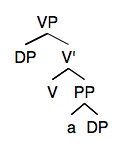
\includegraphics[width=0.9583in,height=1.1252in,width=\textwidth]{sheehan-img001.png}

\end{center}
\begin{center}
 [Warning: Image ignored] % Unhandled or unsupported graphics:
%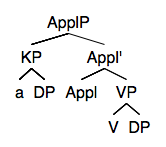
\includegraphics[width=1.3543in,height=1.2083in,width=\textwidth]{sheehan-img002.png}

\end{center}
\begin{styleStandard}
a. \ \ b. 
\end{styleStandard}

\begin{styleStandard}
On these (well-motivated) assumptions, there is al alternative reason that the PCC holds only in the presence of a dative clitic: \ because this element serves to indicate the presence of an Applicative head. The presence of the clitic in (11c-d) therefore indicates a radically different underlying structure, which is not morphologically disambiguated in Italian, French and Catalan.\textstyleFootnoteSymbol{ }\footnote{ Ormazabal and Romero (2013) offer a different competition-based account of this pattern whereby the two a-marked DPs compete for the same Case position in spec vP. Space precludes a full discussion, but, while attractive, it seems that their account cannot be extended to the causative data to be discussed below, where the PCC holds with full DPs even in the absence of clitic doubling.}\ In order to ascertain whether the PCC is sensitive only to this structural difference or to the presence of the dative clitic itself, we need a context in which an indirect object marked with ‘a/à’ is not clitic doubled but cannot function as a locative. If the PCC holds in such contexts then we will know that the weak status of the indirect object is not crucial to the PCC. In the following section I show that the faire infinitive causative is such a context, and that in such cases the PCC can be observed to hold of all datives, not just clitics.
\end{styleStandard}

\begin{stylelsSectioni}
3. The PCC in causatives
\end{stylelsSectioni}

\begin{styleStandard}
A consideration of causatives shows that the PCC data for French, Italian and Catalan in ditransitive contexts are actually misleading. As Bonet (1991) and others have noted, the PCC (somewhat unsurprisingly) also holds with dative clitic causees in the \textit{faire-infinitive} (Postal 1981; Quicoli 1984, Rezac 2008):\footnote{ I use the term ‘faire infinitive’ here to denote a particular kind of Romance causative, following Kayne (1975). Its crucial properties include: (i) dative on transitive causees, (ii) VS order for the caused event, (iii) causees which are agentive and (iv) causers which are not. Space precludes a discussion of minor differences between languages and I merely adopt the most uncontroversial account here, for expository reasons. }
\end{styleStandard}

\begin{styleStandard}
(\stepcounter{qwerty}{\theqwerty})\ \ French (Rezac 2008: 66, citing Postal 1981, Quicoli 1984)
\end{styleStandard}

\begin{styleStandard}
\ \ *Je \ \ vous \ \ \ \ lui \ \ \ \ \ \ \ \ \ \ laisserai \ \ voir
\end{styleStandard}

\begin{styleStandard}
\ \ \ \ I \ \ \ \ \ you.\textsc{acc}= \ \ \ \ her.\textsc{dat=} \ \ let.3\textsc{s}.\textsc{fut} \ \ \ see
\end{styleStandard}

\begin{styleStandard}
\ \ Intended: ‘I will let her see you. 
\end{styleStandard}

\begin{styleStandard}
As Bonet further notes, however, following Postal (1989), full DP datives are also banned in the presence of first/second person direct objects in this context in French:
\end{styleStandard}

\begin{styleStandard}
(\stepcounter{qwerty}{\theqwerty})\ \ French (Postal 1989: 2)
\end{styleStandard}

\begin{styleStandard}
\ \ a.\ \ *Marcel vous \ \ a \ \ fait \ \ épouser \ \ au \ \ \ \ médecin.
\end{styleStandard}

\begin{styleStandard}
\ \ \ \ Marcel \ \ you.\textsc{acc}=\ \ has \ \ made \ \ marry \ \ to.the \ \ doctor
\end{styleStandard}

\begin{styleStandard}
\ \ \ \ Intended: ‘Marcel had the doctor marry you.’
\end{styleStandard}

\begin{styleStandard}
\ \ b. \ \ *On \ \ nous \ \ \ \ a \ \ fait \ \ \ \ choisir \ \ à Jacques
\end{styleStandard}

\begin{styleStandard}
\ \ \ \ one \ \ \ \ us.\textsc{acc} =has \ \ made \ \ choose \ \ to Jacques
\end{styleStandard}

\begin{styleStandard}
\ \ Intended: ‘One/we had Jacques choose us.’
\end{styleStandard}

\begin{styleStandard}
\ \ c. \ \ *On \ \ vous \ \ laissera \ \ connaître \ \ à Louise.
\end{styleStandard}

\begin{styleStandard}
\ \ \ \ one \ \ you\textsc{.acc}=\ \ let.\textsc{3s.fut} know \ \ \ \ to Louise
\end{styleStandard}

\begin{styleStandard}
\ \ \ \ ‘We will let Louise meet you.
\end{styleStandard}

\begin{styleStandard}
These kinds of examples contrast minimally with examples involving a 3\textsuperscript{rd} person direct object (even an animate one), which are fully grammatical, as Postal notes:
\end{styleStandard}

\begin{styleStandard}
(\stepcounter{qwerty}{\theqwerty})\ \ French (Postal 1989: 2)
\end{styleStandard}

\begin{styleStandard}
\ \ a.\ \ Marcel \ \ l’ \ \ \ \ \ \ a\ \ fait\ \ \ \ épouser \ \ au \ \ \ \ médecin.
\end{styleStandard}

\begin{styleStandard}
\ \ \ \ Marcel \ \ her\textsc{.acc} =\ \ has\ \ made\ \ \ \ marry \ \ to.the \ \ doctor
\end{styleStandard}

\begin{styleStandard}
\ \ \ \  ‘Marcel had the doctor marry her.’
\end{styleStandard}

\begin{styleStandard}
b. \ \ On \ \ les \ \ \ \ \ \ a \ \ fait \ \ \ \ choisir \ \ à Jacques
\end{styleStandard}

\begin{styleStandard}
\ \ \ \ one \ \ them.\textsc{acc}=\ \ has \ \ made \ \ choose \ \ to Jacques
\end{styleStandard}

\begin{styleStandard}
\ \  ‘We had Jacques choose them.’
\end{styleStandard}

\begin{styleStandard}
Postal calls this the ‘Fancy Constraint’ and perhaps for this reason it is not usually discussed in connection with the PCC. It is, however, essentially a simpler version of the PCC, which we will call the ‘Simpler PCC’:
\end{styleStandard}

\begin{styleStandard}
(\stepcounter{qwerty}{\theqwerty})\ \ Simpler PCC (first version)
\end{styleStandard}

\begin{listWWNumxxiileveli}
\item 
\begin{listWWNumxxiilevelii}
\item 
\begin{listWWNumxxiileveliii}
\item 
\begin{listWWNumxxiileveliv}
\item 
\begin{styleListParagraph}
In a combination of a direct object and dative in a causative construction, the direct object has to be third person.
\end{styleListParagraph}
\begin{styleListParagraph}
If the direct object is phonologically weak. 
\end{styleListParagraph}
\end{listWWNumxxiileveliv}
\end{listWWNumxxiileveliii}
\end{listWWNumxxiilevelii}
\end{listWWNumxxiileveli}
\begin{styleStandard}
I call (16) ‘simpler’ because it imposes no requirement on the status of the indirect object. This is the version of the PCC which holds also in Catalan and Italian causatives (the Catalan example is from Bonet and the Italian example from my own informants). 
\end{styleStandard}

\begin{styleStandard}
(\stepcounter{qwerty}{\theqwerty})\ \ Catalan (Bonet 1991: 195)
\end{styleStandard}

\begin{styleStandard}
\ \ *Em \ \ \ \ \ \ van \ \ \ \ fer \ \ \ \ escollir \ \ a \ \ la \ \ Teresa
\end{styleStandard}

\begin{styleStandard}
\ \ \ \ me.\textsc{acc}=\ \ go.\textsc{3pl \ \ }make \ \ choose \ \ to \ \ the \ \ Teresa
\end{styleStandard}

\begin{styleStandard}
‘They made Teresa choose me.’
\end{styleStandard}

\begin{styleStandard}
(\stepcounter{qwerty}{\theqwerty})\ \ Italian 
\end{styleStandard}

\begin{styleStandard}
\ \ *Ti \ \ \ \ ho \ \ \ \ fatto \ \ picchiare \ \ \ \ a \ \ mio \ \ fratello
\end{styleStandard}

\begin{styleStandard}
\ \ You.\textsc{acc}\ \ have.\textsc{1sg} \ \ made beat \ \ \ \ \ \ \ \ to \ \ my \ \ brother
\end{styleStandard}

\begin{styleStandard}
\ \  \ Intended: ‘I made my brother beat you.’
\end{styleStandard}

\begin{styleStandard}
The same effect can be observed in Spanish (both Peninsular and Rioplatense), though it is more difficult to observe because of the additional availability of an ECM construction with these verbs (see Strozer 1976, Torrego 2010). Because of these complications, I discuss Spanish in a separate section below. \ 
\end{styleStandard}

\begin{styleStandard}
As Postal also notes, the Fancy Constraint holds only where the causee is dative, and not where it is introduced by a preposition like \textit{par/de} or where no causee is overtly expressed:
\end{styleStandard}

\begin{styleStandard}
(\stepcounter{qwerty}{\theqwerty})\ \ French (Postal 1989: 3)
\end{styleStandard}

\begin{styleStandard}
\ \ a. \ \ Marcel vous \ \ \ \ a\ \ fait \ \ épouser \ \ par \ \ le \ \ médecin.
\end{styleStandard}

\begin{styleStandard}
\ \ \ \ Marcel you.\textsc{acc}=\ \ has\ \ made \ \ marry \ \ by \ \ the \ \ doctor
\end{styleStandard}

\begin{styleStandard}
\ \ \ \ ‘Marcel had the doctor marry you.’
\end{styleStandard}

\begin{styleStandard}
b. \ \ On\ \ nous \ \ \ \ a \ \ fait choisir.
\end{styleStandard}

\begin{styleStandard}
\ \ \ \ One \ \ us.\textsc{acc}\ \ =\ \ has \ \ made choose
\end{styleStandard}

\begin{styleStandard}
\ \ \ \ ‘One/we had us chosen.’
\end{styleStandard}

\begin{styleStandard}
This is further potential evidence that we are dealing with the PCC. Though the structure of the \textit{faire-par} construction remains contested, there is widespread recognition that the ‘by phrase’ in examples like (19a) has adjunct-like properties and is not even projected in (19b) (see Guasti 1996, Folli \& Harley 2007, Sheehan and Cyrino 2016 for recent discussion). In any case, evidence from binding shows that a by-phrase causee does not c-command the accusative object in the \textit{faire-par} construction, whereas a dative causee in the \textit{faire-infinitive} does, as Burzio (1986) shows:
\end{styleStandard}

\begin{styleStandard}
(\stepcounter{qwerty}{\theqwerty})\ \ Italian (Burzio 1986) 
\end{styleStandard}

\begin{styleStandard}
Ho \ \ fatto \ \ riparare \ \ la \ \ propria\textsubscript{i\ \ }macchina\ \ a\ \ Gianni\textsubscript{i}/*da \ \ Gianni\textsubscript{i}
\end{styleStandard}

\begin{styleStandard}
have.1S \ \ made \ \ repair \ \ the\ \ own \ \ car \ \ to \ \ Gianni/\ \ by \ \ Gianni
\end{styleStandard}

\begin{styleStandard}
‘I made Gianni repair his own car.’
\end{styleStandard}

\begin{styleStandard}
In fact, there is evidence that in the \textit{faire-par} construction, c-command relations are reversed, with the accusative object binding into the by-phrase causee (Sheehan \& Cyrino 2016):
\end{styleStandard}

\begin{styleStandard}
(\stepcounter{qwerty}{\theqwerty})\ \ Italian (Sheehan \& Cyrino 2016: 286)
\end{styleStandard}

\begin{styleStandard}
a. \ \ Ho \ \ fatto \ \ leggere [\ \ ogni \ \ libro]\textsubscript{i \ \ }dal \ \ suo\textsubscript{i} \ \ autore. 
\end{styleStandard}

\begin{styleStandard}
\ \ have.1SG \ \ made \ \ read \ \ each book \ \ by.the \ \ its \ \ author\ \ 
\end{styleStandard}

\begin{styleStandard}
\ \ ‘I had each book read by its author.’
\end{styleStandard}

\begin{styleStandard}
b. \ \ *Ho \ \ fatto \ \ leggere \ \ il\ \ suo\textsubscript{i\ \  }libro \ \ da \ \ [ogni\ \ autore]\textsubscript{i}
\end{styleStandard}

\begin{styleStandard}
\ \ have.1SG \ \ made \ \ read \ \ the\ \ his \ \ book \ \ by \ \ each \ \ author
\end{styleStandard}

\begin{styleStandard}
It seems reasonable to assume, then, that the lack of PCC effects in such contexts can be attributed to the fact that the by phrase does not intervene (in c-command terms) between v and the accusative argument. 
\end{styleStandard}

\begin{styleStandard}
The dative causee in the \textit{faire-infinitive,} however, is argument-like, obligatory and merged in a position which c-commands the accusative internal argument. This is reflected by the anaphor binding pattern in (20). Folli \& Harley (2007) propose that dative causees are merged in a righthand specifier of a lower vP, a proposal which I adopt here for ease of exposition, though other options are possible. In Italian and French, at least, all accusative and dative clitics must cliticise onto the causative verb (Kayne 1975, Burzio 1986, Guasti 1993). If cliticization is mediated by Agree, as Preminger (2019) claims, then a defective intervention configuration clearly arises as the FARE verb which I take to be an instance of a higher v, is clearly higher than the causee. The direct object clitic \textit{lo} is therefore c-commanded by v and ‘a Gianni,’ and ‘a Gianni’ is c-commanded by the higher FARE v, despite the unmarked word order:
\end{styleStandard}

\begin{styleStandard}
(\stepcounter{qwerty}{\theqwerty})\ \ Basic structure of faire-infinitive
\end{styleStandard}

\begin{styleStandard}

\end{styleStandard}

\begin{center}
 [Warning: Image ignored] % Unhandled or unsupported graphics:
%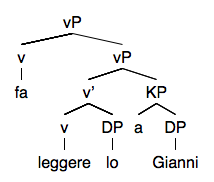
\includegraphics[width=1.8307in,height=1.5591in,width=\textwidth]{sheehan-img003.png}

\end{center}
\begin{styleStandard}
Postal proposes that, while the Fancy Constraint is widespread in French, it is not observed where the verbal complement of \textit{faire} is headed by \textit{connaître/reconnaître} or \textit{voir}, providing the following data:
\end{styleStandard}

\begin{styleStandard}
(\stepcounter{qwerty}{\theqwerty})\ \ French (Postal 1989: 4)
\end{styleStandard}

\begin{styleStandard}
\ \ a. \ \ On \ \ vous \ \ \ \  fera \ \ \ \ \ \ \ \ connaître \ \ à Louise.
\end{styleStandard}

\begin{styleStandard}
\ \ one \ \ you.\textsc{acc}=make.\textsc{3sg.fut} \ \ know \ \ \ \ to Louise
\end{styleStandard}

\begin{styleStandard}
\ \ ‘We made Louise meet you.’
\end{styleStandard}

\begin{styleStandard}
b. \ \ Jacques nous \ \ \ \ a \ \ \ \ fait \ \ voir \ \ à ses chefs
\end{styleStandard}

\begin{styleStandard}
\ \ \ \ Jacques us.\textsc{acc} =\ \ has \ \ made see \ \ to his bosses
\end{styleStandard}

\begin{styleStandard}
\ \ \ \ ‘Jacques made his bosses see us.’
\end{styleStandard}

\begin{styleStandard}
This is a potentially important distinction, which might shed important light on the nature of the PCC, if robust. Judgments on such are examples are varied, however and, although the effect might be less categorical than with other verbs, experimental results suggest that at least with \textit{voir}, the PCC still holds in its simpler form.
\end{styleStandard}

\begin{styleStandard}
Given the sensitivity of judgments of this kind, 14 examples of this kind were included as fillers (with a parallel context) in a large online survey, taken by 42 people. Questions were presented in randomized order and rated on an 8-point scale from 0-7. Mean scores are given across participants. The results show a clear contrast: examples with 3rd person direct objects were clearly grammatical, receiving an average of acceptability of just under 5, regardless of the features of the indirect object (17). Examples with two clitics received a slightly lower average mean (17b), probably for processing reasons. All examples were presented along with a context (given in French) set in a busy classroom at the beginning of the school year:
\end{styleStandard}

\begin{styleStandard}
(\stepcounter{qwerty}{\theqwerty})\ \ French non-PCC contexts of \textit{faire-voir} ‘show’ 
\end{styleStandard}

\begin{styleStandard}
\ \ a. \ \ La \ \ professeure \ \ \textbf{te/\ \ lui/\ \ me} \ \ \ \ fait \ \ \ 
\end{styleStandard}

\begin{styleStandard}
\ \ \ \ the \ \ teacher \ \ you.\textsc{dat}/her.\textsc{dat}/me.\textsc{dat}= makes 
\end{styleStandard}

\begin{styleStandard}
\ \ \ \ voir \textbf{Jean},\ \ qui \ \ se \ \ sent \ \ nerveux. 
\end{styleStandard}

\begin{styleStandard}
\ \ \ \ see \ \ Jean, \ \ who \textsc{se} \ \ feels \ \ nervous
\end{styleStandard}

\begin{styleStandard}
\ \ ‘The teacher shows you/her/me Jean, who is feeling nervous.’\ \ \ \ \ \ \ \ \textbf{[mean rating: 4.98/4.86/4.62]}
\end{styleStandard}

\begin{styleStandard}
b. \ \ La \ \ professeure \ \ \textbf{me \ \ le}\ \ fait\ \ voir. \ \ 
\end{styleStandard}

\begin{styleStandard}
\ \ \ \ the \ \ teacher\ \ me.\textsc{dat=}him.\textsc{acc=}\ \ makes\ \ see
\end{styleStandard}

\begin{styleStandard}
\ \ \ \ ‘The teacher shows me him.’ \ \ \textbf{[mean rating: 4.45]}
\end{styleStandard}

\begin{styleStandard}
This is as expected as these are non-PCC contexts in French because the direct object in all cases is 3\textsuperscript{rd} person. 
\end{styleStandard}

\begin{styleStandard}
There is a clear contrast when we consider examples with 1st/2nd person direct object and a 3\textsuperscript{rd} person causee, the ‘strong PCC’ context. These were most unacceptable with dative clitics (25a), but were also rated very low with full DP datives (an average of around 2 on the scale 8-point scale)(25b):
\end{styleStandard}

\begin{styleStandard}
(\stepcounter{qwerty}{\theqwerty})\ \ French PCC contexts of \textit{faire-voir} ‘show’
\end{styleStandard}

\begin{styleStandard}
\ \ a. \ \ *Le professeur\ \ \textbf{me/ \ \ te \ \ \ \ \ \ lui} \ \ fait \ \ voir. 
\end{styleStandard}

\begin{styleStandard}
\ \ \ \ the \ \ teacher\ \ me.\textsc{acc/}\ \ you.\textsc{acc}=\ \ him.\textsc{dat}=\ \ make see
\end{styleStandard}

\begin{styleStandard}
Intended: ‘The teacher shows me/you to him.’
\end{styleStandard}

\begin{styleStandard}
\textbf{[mean~ratings: 0.49/0.50]}
\end{styleStandard}

\begin{styleStandard}
\ \ b. \ \ *?La \ \ professeure \ \ \textbf{me/\ \ \ \ te} \ \ \ \ \ \ fait \ \ \ \ voir 
\end{styleStandard}

\begin{styleStandard}
\ \ \ \ the \ \ \ \ teacher \ \ \ \ me.\textsc{acc}/\ \ you.\textsc{acc=} makes \ \ see 
\end{styleStandard}

\begin{styleStandard}
à \ \ Marie,\ \ qui \ \ se\ \ sent \ \ à \ \ l’\ \ aise. 
\end{styleStandard}

\begin{styleStandard}
to Marie, who \textsc{se} \ \ feels \ \ at \ \ the ease
\end{styleStandard}

\begin{styleStandard}
Intended: ‘The teacher shows you to Marie, 
\end{styleStandard}

\begin{styleStandard}
who is feeling at ease.’\ \ \textbf{[mean~ratings: 1.79/2.05]}
\end{styleStandard}

\begin{styleStandard}
While further empirical investigation of the kinds of contrasts noted by Postal with individual verbs is clearly warranted, these initial experimental data suggest that the simpler PCC also holds with full dative DPs even where the embedded verb is \textit{voir}. 
\end{styleStandard}

\begin{styleStandard}
The implication of the Catalan, Italian and French causative patterns is that the PCC in Romance languages is \textit{not} limited to contexts where the indirect object is a clitic or an element triggering morphological agreement. The languages in question fail to have clitic doubling of datives and yet the PCC still holds even where the dative is a full DP. In this way, the data show that the PCC holds wherever (i) the direct object has the relevant (language-specific) person/animacy feature; (ii) v establishes a detectable Agree relation with this direct object and (iii) an indirect object of any kind intervenes in that Agree relation. This can lead either to ungrammaticality (strong PCC) or interaction between phi-features (weak PCC). \ 
\end{styleStandard}

\begin{styleStandard}
There is evidence that Postal’s Fancy Constraint is just the PCC from the kinds of repairs which are available in this context. Recall that in ditransitive contexts, changing a dative clitic into a tonic pronoun marked with a/à served to repair the PCC. In causative contexts, PCC violations can only be repaired by making the \textit{direct} object into a tonic pronoun:
\end{styleStandard}

\begin{styleStandard}
(\stepcounter{qwerty}{\theqwerty})\ \ French
\end{styleStandard}

\begin{styleStandard}
Je \ \ n’\ \ ai \ \ fait \ \ frapper \ \ que \ \ toi \ \ à \ \ Jean
\end{styleStandard}

\begin{styleStandard}
\ \ I \ \ \textsc{neg} \ \ have \ \ made \ \ hit \ \ but \ \ you \ \ to \ \ Jean
\end{styleStandard}

\begin{styleStandard}
\ \ ‘I only made Jean hit YOU.’
\end{styleStandard}

\begin{styleStandard}
(\stepcounter{qwerty}{\theqwerty})\ \ Italian
\end{styleStandard}

\begin{styleStandard}
Ho \ \ \ \ \ \ fatto \ \ picchiare \ \ TE\ \ a\ \ mio\ \ fratello
\end{styleStandard}

\begin{styleStandard}
\ \ have.\textsc{1sg} \ \ made \ \ beat \ \  \ \ YOU\ \ to\ \ my\ \ brother
\end{styleStandard}

\begin{styleStandard}
\ \ ‘I made my brother beat YOU.’
\end{styleStandard}

\begin{styleStandard}
But, unlike in ditransitive contexts, changing the status of the dative does not help here: tonic pronouns are also banned in the presence of 1st/2nd person direct object clitics, just as full dative DPs are:
\end{styleStandard}

\begin{styleStandard}
(\stepcounter{qwerty}{\theqwerty})\ \ Italian\footnote{ Another possible repair for some Italian speakers is to make the causee accusative, giving rise to an ECM-type complement without clitic climbing (Schifano \& Sheehan 2017):\par \par 
\setcounter{listWWNumxxvleveli}{0}
\begin{listWWNumxxvleveli}
\item 
\begin{styleListParagraph}
\%Lo/ *gli \ \ \ \ \ fece \ \ \ \ \ picchiarmi
\end{styleListParagraph}
\end{listWWNumxxvleveli}
\ \ \ \ 3sg.acc/ \ 3sg.dat made \ \ \ beat.inf.=1sg.acc\ \ \par \ \ \ \ ‘She made him beat me’\par \par ECM is not usually possible with Italian FARE (but see Burzio 1986, Schifano \& Sheehan 2017 for discussion). This repair is not possible with full DP causees, for unclear reasons, making it only partially parallel to what is described for Spanish below. }
\end{styleStandard}

\begin{styleStandard}
*Ti ho \ \ \ \ \ \ \ fatto \ \ picchiare \ \ a \ \ \ lui/LUI
\end{styleStandard}

\begin{styleStandard}
\ \ you have \ \ made \ \ beat \ \ \ \ to him/HIM
\end{styleStandard}

\begin{styleStandard}
\ \ Intended: ‘I made him/HIM beat you.’
\end{styleStandard}

\begin{styleStandard}
In sum, we have seen that a ‘simper PCC’ applies to causatives such that a 1\textsuperscript{st}/2\textsuperscript{nd} person direct object clitic is ruled out in the presence of any kind of dative in French, Italian and Catalan. Why do the data pattern differently in causative vs. ditransitive contexts? In ditransitive contexts we saw that, with the exception of Spanish (which has clitic doubling), no PCC effect was observed with full DP datives. In section 5, I propose that this is because ditransitives are structurally ambiguous in French, Italian and Catalan, just as they are in Spanish. As we saw for Spanish ditransitives, then, the PCC holds only where a DP is dative and not where it is locative. Before presenting this proposal, however, I discuss the behaviour of Spanish in causative contexts, as these data present additional complications, but essentially serve to reinforce the point being made. 
\end{styleStandard}

\begin{stylelsSectioni}
4. Spanish causatives
\end{stylelsSectioni}

\begin{styleStandard}
According to Torrego (2010), clitic doubling of datives in the faire-infinitive is optional, at least for some Spanish speakers (see also Pineda 2013 regarding ditransitives). I take the VS order in (29) to indicate that this is an instance of the \textit{faire infinitive }nonetheless:
\end{styleStandard}

\begin{styleStandard}
(\stepcounter{qwerty}{\theqwerty})\ \ Spanish (Torrego 2010: 448)
\end{styleStandard}

\begin{styleStandard}
La \ \ entrenadora\ \ (le) \ \ hizo \ \ repetir\ \ el \ \ ejercicio \ \ a \ \ \ \ la \ \ atleta.
\end{styleStandard}

\begin{styleStandard}
the \ \ trainer \ \ (her.\textsc{dat}=) \ \ made \ \ repeat\ \ the \ \ exercise \ \ to \ \ the\ \ athlete
\end{styleStandard}

\begin{styleStandard}
‘The trainer made the athlete repeat the exercise.’
\end{styleStandard}

\begin{styleStandard}
In a PCC context then, a 1\textsuperscript{st}/2\textsuperscript{nd} person clitic is unsurprisingly ruled out in the presence of a clitic doubled dative. Note that this a spurious ‘se’ context in Spanish:
\end{styleStandard}

\begin{styleStandard}
(\stepcounter{qwerty}{\theqwerty})\ \ Spanish
\end{styleStandard}

\begin{styleStandard}
*Marcelo \ \ se \ \ te \ \ hizo \ \ saludar\ \ al \ \ invitado.\ \ 
\end{styleStandard}

\begin{styleStandard}
Marcelo \ \ him.\textsc{dat}=\ \ you.\textsc{acc}=\ \ made \ \ greet\ \ to.the \ \ guest
\end{styleStandard}

\begin{styleStandard}
\ \ ‘Intended: Marcelo made the guest greet you.’
\end{styleStandard}

\begin{styleStandard}
What is more interesting, from our perspective, is what happens where the dative clitic is absent. Examples such as (31a-b) should be potentially ambiguous with either the clitic of the full DP functioning as the causee. This is because, as in the other Romance languages, 1\textsuperscript{st} and 2\textsuperscript{nd} person clitics are not morphologically distinguished for accusative and dative case and because, due to DOM, all animate internal arguments in Spanish are introduced by ‘a’. \ In both cases, however, the 1st/2nd person clitic can only be construed as a dative causee, however:
\end{styleStandard}

\begin{styleStandard}
(\stepcounter{qwerty}{\theqwerty})\ \ Spanish
\end{styleStandard}

\begin{styleStandard}
a. \ \ Marcelo \ \ te \ \ \ \ hizo \ \ \ \ ver \ \ al \ \ médico.
\end{styleStandard}

\begin{styleStandard}
\ \ Marcelo \ \ you.*\textsc{acc/.dat=}\ \ made\ \ see \ \ \ \ to.the \ \ doctor
\end{styleStandard}

\begin{styleStandard}
\ \ (i) ‘Marcelo made you see the doctor.’
\end{styleStandard}

\begin{styleStandard}
\ \ (ii) *‘Marcelo made the doctor see you.’
\end{styleStandard}

\begin{styleStandard}
b. \ \ Nos \ \ \ \ dejará \ \ ver \ \ a \ \ Luisa.
\end{styleStandard}

\begin{styleStandard}
\ \ Us.*\textsc{acc/ dat= \ \ }let.\textsc{fut}\ \ see \ \ to \ \ Luisa
\end{styleStandard}

\begin{styleStandard}
\ \ (i) ‘He made us see Luisa.’
\end{styleStandard}

\begin{styleStandard}
\ \ (ii) *‘He made Luisa see us.’
\end{styleStandard}

\begin{styleStandard}
This is essentially the same effect described for Italian, French and Spanish: it is not possible to have a 1\textsuperscript{st}/2\textsuperscript{nd} person direct object in the presence of a dative argument. The only difference is that the presence of DOM means that the example is not ungrammatical, as the alternative reading in (i) is available. There is much more to be said about Spanish causatives, however. 
\end{styleStandard}

\begin{styleStandard}
In addition to the faire infinitive, many varieties of Spanish appear to permit ECM complements of \textit{hacer} ‘make’. For our purposes, the relevant properties of this type of complement is that: (i) transitive causees can be realised as accusative clitics; (ii) SV order is observed in the caused event; (iii) clitic climbing is not possible (Strozer 1976, Treviño 1992, 1993, Torrego 2010, Tubino Blanco 2011). Consider the following examples by way of illustration of these properties in Mexican Spanish:
\end{styleStandard}

\begin{styleStandard}
(\stepcounter{qwerty}{\theqwerty})\ \ Mexican Spanish (Treviño 1992: 311, 169)
\end{styleStandard}

\begin{styleStandard}
a. \ \ Juan lo \ \ \ \ hizo \ \ leer \ \ estos libros. \ \ \ \ 
\end{styleStandard}

\begin{styleStandard}
Juan him\textsc{.acc}=\ \ made \ \ read \ \ these books
\end{styleStandard}

\begin{styleStandard}
‘Juan made him read these books.’\ \ 
\end{styleStandard}

\begin{styleStandard}
b. \ \ Él\ \ hizo\ \ [\ \ a \ \ Sadat\ \ exportarlas\ \ \ \ \ \ desde \ \ Francia].
\end{styleStandard}

\begin{styleStandard}
He\ \ made\ \ \ \ to \ \ Sadat\ \ export.\textsc{inf}=them.\textsc{acc} \ \ from \ \ France
\end{styleStandard}

\begin{styleStandard}
c. \ \ *Él\ \ las\ \ hizo [\ \ a \ \ Sadat \ \ exportar \ \ desde \ \ Francia].
\end{styleStandard}

\begin{styleStandard}
\ \ he them.\textsc{acc}= \ \ made \ \ to Sadat \ \ export.\textsc{inf} from \ \ France 
\end{styleStandard}

\begin{styleStandard}
Once we accept that in Spanish, unlike in French, Italian and (for the most part) Catalan, an ECM-type of complement is available under the FARE cognate verb, some apparently quirky properties of Spanish causatives can be attributed to the PCC.\footnote{ Actually a minority of Catalan speakers do seem to permit ECM under \textit{fer, }but this is certainly not a majority pattern (see Pineda, Schifano \& Sheehan 2018). \ } 
\end{styleStandard}

\begin{styleStandard}
First, consider the curious fact that animate direct object clitics cannot climb onto the causative verb in Spanish causatives (Rivas 1977, Bordelois 1978, Torrego 2010):
\end{styleStandard}

\begin{styleStandard}
(\stepcounter{qwerty}{\theqwerty})\ \ Spanish (Torrego 2010: 463)
\end{styleStandard}

\begin{styleStandard}
a. \ \ *El \ \ me \ \ \ \ lo \ \ \ \ hizo \ \ saludar.
\end{styleStandard}

\begin{styleStandard}
he \ \ me.\textsc{dat }=\ \ him.\textsc{acc }=\ \ made greet
\end{styleStandard}

\begin{styleStandard}
‘He made me greet him.’
\end{styleStandard}

\begin{styleStandard}
b. \ \ El \ \ me \ \ \ \ hizo \ \ saludarlo.
\end{styleStandard}

\begin{styleStandard}
he \ \ me.\textsc{dat=\ \ }made \ \ greet=him.\textsc{acc}
\end{styleStandard}

\begin{styleStandard}
In the current context, and bearing in mind the fact that Spanish displays PCC effects with animate direct objects, (33a) looks like a PCC effect. If this is the case, then it is not the clitic cluster that is a problem, nor the dative 1\textsuperscript{st} person clitic, but rather the animate direct object which attempts to Agree with \textit{hacer} ‘make’ past the dative causee.\footnote{ As noted above a similar effect is attested with the 3\textsuperscript{rd} person masculine singular animate clitic \textit{le} in \textit{leísta} dialects of Spanish. I am not sure to what extent animate direct object clitics in non-\textit{ leísta }dialects also trigger PCC effects with ditransitives. \textit{\ }} Example (33b) is grammatical, however, because it involves a more biclausal ECM construction in which the accusative clitic does not form an Agree dependency with \textit{hacer}, but rather with the lexical verb \textit{saludar}. As the causee asymmetrically c-commands this lexical verb, it does not function as an intervener in (33b). 
\end{styleStandard}

\begin{styleStandard}
\ \ As this ECM causative is ‘biclausal’ in the relevant sense, it also fails to be subject to more standard PCC effects. Speakers of Latin American varieties of Spanish and many Peninsular varieties readily accept examples such as the following:
\end{styleStandard}

\begin{styleStandard}
(\stepcounter{qwerty}{\theqwerty})\ \ Spanish
\end{styleStandard}

\begin{styleStandard}
a. (?) \ \ Marcelo \ \ hizo \ \ al \ \ invitado\ \ saludarte.\newline
\ \ \ \ Marcelo \ \ made\ \ to.the \ \ guest \ \ greet=you.\textsc{acc}
\end{styleStandard}

\begin{styleStandard}
\textsc{\ \ \ \ ‘}Marcelo made the guest greet you.’
\end{styleStandard}

\begin{styleStandard}
b. (?) Dejará \ \ a \ \ Luisa \ \ vernos.\newline
 \ \ \ \  let.\textsc{fut} \ \ to \ \ Luisa \ \ see=us.\textsc{acc}
\end{styleStandard}

\begin{styleStandard}
\ \ ‘They will let Luisa see us.’
\end{styleStandard}

\begin{styleStandard}
These examples clearly have an interpretation whereby the 1\textsuperscript{st}/2\textsuperscript{nd} person clitic is construed as a direct object, as indicated in the gloss, and so there is no PCC effect in evidence. Again, this is because the direct object clitic does not agree with the matrix little v. In this way, PCC effects in Spanish causatives are more nuanced than in the other Romance languages under discussion. 
\end{styleStandard}

\begin{styleStandard}
Now consider examples involving an animate direct object with DOM. As discussed above, these kinds of direct objects trigger PCC effects in Spanish ditransitives in the presence of clitic doubling, as discussed above. With causatives, the pattern is slightly different:
\end{styleStandard}

\begin{styleStandard}
(\stepcounter{qwerty}{\theqwerty})\ \ Spanish
\end{styleStandard}

\begin{styleStandard}
\ \ a. \ \ *Ana \ \ hizo \ \ saludar \ \ a \ \ su \ \ marido \ \ al\ \ \ \ invitado
\end{styleStandard}

\begin{styleStandard}
\ \ \ \ Ana \ \ made \ \ greet \ \ to \ \ her \ \ husband\ \ to.the \ \ guest\ \ 
\end{styleStandard}

\begin{styleStandard}
\ \ b. \ \ *Ana \ \ le \ \ hizo \ \ saludar \ \ a \ \ su \ \ marido \ \ al \ \ invitado
\end{styleStandard}

\begin{styleStandard}
\ \ Ana \ \ him.dat \ \ made \ \ greet \ \ to \ \ her husband to.the \ \ guest
\end{styleStandard}

\begin{styleStandard}
c. \ \ Ana \ \ hizo \ \ \ \ al \ \ \ \ invitado \ \ saludar \ \ a \ \ su \ \ marido.
\end{styleStandard}

\begin{styleStandard}
\ \ Ana \ \ made \ \ to.the \ \ guest \ \ greet \ \ to \ \ her \ \ husband
\end{styleStandard}

\begin{styleStandard}
d. \ \ \%Ana le \ \ hizo \ \ al \ \ invitado saludar \ \ a \ \ \ \ su \ \ marido.
\end{styleStandard}

\begin{styleStandard}
\ \ Ana \ \ him.dat \ \ made \ \ to.the \ \ guest \ \ greet \ \ to \ \ her \ \ husband
\end{styleStandard}

\begin{styleStandard}
\ \ ‘Ana made the guest greet her husband.’
\end{styleStandard}

\begin{styleStandard}
If we take the basic position of the causee to indicate the difference between the faire-infinitive and ECM causatives, then these data show that PCC holds with DOM-marked full DP direct objects in the faire infinitive regardless of whether the indirect object is clitic doubled. In (35a-b), the VS order in the caused event indicates that this is an instance of the faire-infinitive, with clause union. For this reason, a DOM-marked direct object is not possible, by hypothesis, because the dative blocks agreement with the causative verb. Crucially, this is true not only in (35b), where we see clitic doubling of the dative parallel to what we saw with ditransitives, but also in (31a), where there is no dative clitic. This follows if, as noted above, clitic doubling is optional in the Spanish faire-infinitive (see also Pineda 2013, who claims this is true also in Spanish ditransitives). Regardless of clitic doubling, then, the presence of a dative causee will trigger a PCC effect. As described in (12) above, in ditransitive constructions, a non-doubled indirect object has the option of being interpreted as a locative, and it is this fact which makes the presence of a clitic crucial to the PCC in this context. The same is not true in the faire infinitive, where DPs introduced by a/à always have the status of datives, base generated between the direct object and the causative v. 
\end{styleStandard}

\begin{styleStandard}
Now consider (35c-d), which have SV order in the caused event and so can be taken to be instances of ECM causatives. All speakers accept (35c), and this is as expected if this is a biclausal ECM context. Additionally, however, speakers from Argentina and certain parts of Spain also allow (35d). In fact, these speakers also allow, even prefer, clitic doubling of the ECM causee with clitic direct objects, even in ‘strong PCC’ contexts, with 1\textsuperscript{st}/2\textsuperscript{nd} person direct objects:
\end{styleStandard}

\begin{styleStandard}
(\stepcounter{qwerty}{\theqwerty})\ \ Spanish 
\end{styleStandard}

\begin{styleStandard}
a. \ \ \%Marcelo \ \ le \ \ hizo \ \ al \ \ invitado saludarte.\ \ \ \ Marcelo \ \ him.\textsc{dat=} \ \ made \ \ to.the \ \ guest\ \ greet=you.\textsc{acc}
\end{styleStandard}

\begin{styleStandard}
\ \ ‘Marcelo made the guest greet you.’
\end{styleStandard}

\begin{styleStandard}
b. \ \ \%Clara \ \ le \ \ hizo \ \ al \ \ invitado \ \ saludarlo.\ \ \ \ \newline
\ \ Clara \ \ him.\textsc{dat=} made \ \ to.the \ \ guest \ \ greet=him.\textsc{acc}
\end{styleStandard}

\begin{styleStandard}
\ \ \ \ ‘Clara made the guest greet him.’
\end{styleStandard}

\begin{styleStandard}
I leave open the status of the matrix dative clitic is in such examples. The fact that such examples are not subject to the PCC suggests that they cannot be instances of the faire-infinitive with a fronted causee. Ormazabal and Romero (2013) analyse them as instances of raising to object. It still remains unclear to me, however, how a dative clitic doubles an accusative causee (see also Ordóñez and Saab 2018 for one proposal). What is clear from these data, however, despite the open questions, is that Spanish also displays PCC effects with both clitic and full DP datives, in parallel with the other Romance languages under discussion, once we control for the availability of ECM (or raising to object) complements.
\end{styleStandard}

\begin{stylelsSectioni}
5. Theoretical implications
\end{stylelsSectioni}

\begin{styleStandard}
Early approaches to the PCC characterised it as a morphological constraint (see Bonet 1991, for example). More recently, however, significant challenges have been raised for this position (see Preminger 2019 for an overview), and the facts discussed here can be seen as further evidence that the PCC is not about morphology. In fact, the main aim of this chapter has been to show that the relevance of the PCC is \textit{not} limited to clitic clusters in Romance. As we have seen, when we consider Spanish DOM-marked direct objects and \textit{faire-infinitive} causatives, the PCC can be shown not to care about the weak/strong status of the indirect object. All that matters is the syntactic structure and the agreeing status of the direct object. 
\end{styleStandard}

\begin{styleStandard}
While there have been many syntactic analyses of the PCC, most recent approaches reduce to the idea that it arises where “two arguments are in the domain of a single probing head” (Nevins 2007: 290). A line of research stemming from Anagnostopoulou (2003, 2005) formalizes this in terms of defective intervention, whereby a probe attempts to agree with a goal with person features over a dative intervener (see Anagnostopoulou 2003, 2005, Nevins 2007, Rezac 2008, Preminger 2019). A distinct, but related approach, by Adger and Harbour (2007) attributes the PCC to the fact that a single head with one set of person features cannot both agree with an animate [+participant] Theme and introduce an animate [+participant] argument in its specifier as these functions both require a distinct person feature. Note that, in their system, 3\textsuperscript{rd} person Themes are always [-participant], whereas animate recipients/benefactives are [+participant] even if they are 3\textsuperscript{rd} person. \ Both kinds of approaches rely crucially on the fact that the direct object must Agree with a functional head. In the defective intervention approach, this is a head higher than the dative, such as v. In Adger and Harbour’s alterative account, it is Appl, the same head which introduces the applied argument. 
\end{styleStandard}

\begin{styleStandard}
Bianchi (2006) and Stegovec (2017), on the other hand, provide analyses which aim to capture the fact that (in ditransitives) the PCC only holds if both internal arguments are weak elements. In Stegovec’s (2017) approach, for example, weak arguments enter the derivation without a person feature and must receive one via agreement with a phase head. As the indirect object generally intervenes between the direct object and the phase head v, this leads to an intervention problem wherever both are weak 1\textsuperscript{st}/2\textsuperscript{nd} person pronouns. The Spanish data in ditransitives are already problematic for these latter kinds of accounts, as are the Romanian facts presented by Cornilescu (this volume, section 6), and the causative patterns show quite clearly that, in Romance at least, this kind of approach makes the wrong predictions. 
\end{styleStandard}

\begin{styleStandard}
Mainstream accounts can, however, easily accommodate the Simpler PCC defended here. In the defective intervention approach, based on Anagnostopoulou (2003, 2005), Béjar \& Rezac (2003) and Rezac (2008), the PCC arises because a dative argument intervenes between a probe (v) and its [+person] goal, the accusative direct object:
\end{styleStandard}

\begin{styleStandard}
(\stepcounter{qwerty}{\theqwerty})\ \ v\textsubscript{[phi: ]}\ \ \ \ {\textgreater} DP\textsubscript{DAT} {\textgreater} \ \ \ \ DP\textsubscript{[+person]}
\end{styleStandard}

\begin{styleStandard}
On this kind of approach, it is actually mysterious why the PCC would only apply to dative clitics. For the defective intervention account to extend to causatives, it has to be the case that the internal argument of the embedded predicate agrees with \textit{fare}, with the causee acting as an intervener:
\end{styleStandard}

\begin{styleStandard}
(\stepcounter{qwerty}{\theqwerty})\ \ fare\textsubscript{[phi: ]} \ \ {\textgreater}\ \ DP\textsubscript{DAT} {\textgreater} \ \ DP\textsubscript{[+person]}
\end{styleStandard}

\begin{styleStandard}
Given that internal arguments obligatorily cliticise onto \textit{faire}/\textit{fare} in both French and Italian, this kind of analysis seems promising. 
\end{styleStandard}

\begin{styleStandard}
On Adger and Harbour’s (2007) approach, as noted above, the basic prediction is also that there would be no sensitivity to the clitic/non-clitic distinction, just as there is no sensitivity to the case-marking of the higher argument. For them, the PCC arises where a single head must both agree with the internal [+participant] direct object and introduce an animate [+participant] specifier:
\end{styleStandard}

\begin{styleStandard}
(\stepcounter{qwerty}{\theqwerty})\ \ *[\textsubscript{ApplP} DP\textsubscript{[+participant]} Appl … DP\textsubscript{[+participant]}]
\end{styleStandard}

\begin{styleNormalWeb}
This leads to ungrammaticality because a given head can only enter into an Agree relation with the same feature once, and the spec-head relation is conceived of as Agree-based. Whichever head introduces the causee in the faire infinitive: \textit{Appl} (Ippolito 2000, Ordóñez 2008, Torrego 2010, Pitteroff and Campanini 2014) or\textit{ v} (Folli and Harley 2007), this head will be prevented from agreeing with a [+participant] Theme.\footnote{ Note that it is more controversial to claim that the lowest direct object is Case-licensed by \textit{fare/faire}. Belletti and Rizzi (2012) argue that it is, against Folli and Harley’s (2007) position that it is licensed low. The controversy relates partly to the status of passivisation of the faire-infinitive in Italian and French. As Preminger (2019) shows, it is, in any case, possible, and probably necessary, to restate this kind of account without the need for abstract Case as long as cliticisation involves Agree. }\ \ 
\end{styleNormalWeb}

\begin{styleNormalWeb}
So why, then, does it appear to be the case that the PCC holds only where the dative is a clitic in ditransitive contexts in Romance? The answer, I propose, comes from the two potential structures for ditransitives and the fundamental ambiguity of \textit{a/à} as a dative/locative marker, discussed above in relation to Spanish. Following Holmberg, Sheehan and van der Wal (2017) and Fournier (2010), we propose that (like Spanish) Catalan, Italian and French have two distinct structures for ditransitives (see Demonte 1995, Cuervo 2003, Harley 2002, Harley and Miyagawa 2017). These are as illustrated above by (12), repeated here as (40):
\end{styleNormalWeb}

\begin{styleStandard}
(\stepcounter{qwerty}{\theqwerty})\ \ Structures for the double object construction (a) and the prepositional dative (b)
\end{styleStandard}

\begin{styleStandard}

\end{styleStandard}

\begin{center}
 [Warning: Image ignored] % Unhandled or unsupported graphics:
%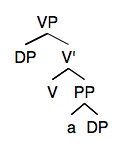
\includegraphics[width=0.9583in,height=1.1252in,width=\textwidth]{sheehan-img001.png}

\end{center}
\begin{center}
 [Warning: Image ignored] % Unhandled or unsupported graphics:
%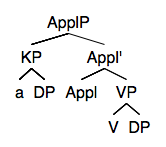
\includegraphics[width=1.3543in,height=1.2083in,width=\textwidth]{sheehan-img002.png}

\end{center}
\begin{styleStandard}
a. \ \ b. 
\end{styleStandard}

\begin{styleStandard}
In the extensive literature on the topic, it has been argued that many unrelated languages permit both kinds of structures, regardless of surface case morphology (see Marantz 1993, Pesetsky 1995, Cuervo 2003, Anagnostopoulou 2003, Pylkkänen 2002, 2008, Miyagawa and Tsujioka 2004, Bruening 2010, Harley \& Miyagawa 2017). The issue remains contentious, however, as several of the other papers in this volume shows, see, especially, Calindro (this volume) and Cépeda \& Cyrino (this volume) on Brazilian Portuguese, Cornilescu (this volume) on Romanian, and Antonyuk (this volume) on Russian. If the Romance languages under discussion have two structures for distransitives, as outlined above, then PCC effects are predicted to hold only in structures like (40a) and not in those like (40b) (see Rezac 2008 on parallel contrasts in Basque). It is only in configurations like (40a) that the indirect object will function as an intervener. Where \textit{a/à} is the head of a locative PP which is base generated below the accusative direct object, no intervention effect will arise. 
\end{styleStandard}

\begin{styleStandard}
In other words, it is this structural ambiguity in ditransitives which gives rise the false impression that the PCC only holds with dative clitics. Full DPs introduced by \textit{a/à }which occur with ditransitive verbs can be either dative or locative, having either the structure in (40a) or that in (40b), whereas dative clitics are unambiguously dative, and so must derive from the structure in (40a)\footnote{ For concreteness, I assume that clitics originate in argument positions, but there are other possibilities. }. Consider, by way of illustration, the French examples in (2)-(3) above, repeated here as (41a-b): 
\end{styleStandard}

\begin{styleStandard}
(\stepcounter{qwerty}{\theqwerty})\ \ French (Kayne 1975: 173, 174)
\end{styleStandard}

\begin{styleStandard}
\ \ a. \ \ \ *Paul \ \ me \ \ \ \ \ \ lui \ \ \ \ \ \ présentera.
\end{styleStandard}

\begin{styleStandard}
\ \ \ \ \ \ Paul \ \ me.\textsc{acc}= \ \ him.\textsc{dat=} present.\textsc{3sg.fut}
\end{styleStandard}

\begin{styleStandard}
\ \ \ \ Intended: ‘Paul will introduce me to him.’
\end{styleStandard}

\begin{styleStandard}
b. \ \ Paul \ \ me \ \ \ \ présentera \ \ \ \ à lui.
\end{styleStandard}

\begin{styleStandard}
\ \ \ \ Paul\ \ me.\textsc{acc}=\ \ present.\textsc{3s.fut} \ \ to him
\end{styleStandard}

\begin{styleStandard}
\ \ \ \ ‘Paul will introduce me to him.’
\end{styleStandard}

\begin{styleStandard}
Example (41a) is ungrammatical because it must have the structure in (40a), whereby the dative intervenes between v and the direct object (in its base position). Example (41b), however, is grammatical because it can be construed with the structure in (40b). I assume that, with the structure in (40a), it is also ungrammatical, in parallel with (41a), and so only (40b) is possible (see also Anagnostopoulou 2003, Rezac 2008 for similar proposals). 
\end{styleStandard}

\begin{styleStandard}
Further support for this view comes from the fact that in French and Catalan the indirect object can be (exceptionally) realised as a locative clitic as a PCC repair strategy (see Postal 1990, Rezac 2008, on French; Bonet 1991, 2007 on Catalan):
\end{styleStandard}

\begin{styleStandard}
(\stepcounter{qwerty}{\theqwerty})\ \ French
\end{styleStandard}

\begin{styleStandard}
\ \ \%\ \ Paul \ \ m’ \ \ \ \ \ \ y \ \ \ \ \ \ présentera.
\end{styleStandard}

\begin{styleStandard}
\ \ \ \ Paul \ \ me.\textsc{acc}= \ \ there\textsc{=} \ \ present.\textsc{3sg.fut}
\end{styleStandard}

\begin{styleStandard}
\ \ ‘Paul will introduce me to him.’
\end{styleStandard}

\begin{styleStandard}
What is usual about such examples is that the locative clitics cannot unusually index animate arguments. Presumably, this is exceptionally permitted in such contexts to avoid ungrammaticality.
\end{styleStandard}

\begin{styleStandard}
More generally, this proposal sheds new light on one of the main kinds of PCC repairs: they simply involve the prepositional dative construction not a PF repair. This explains immediately why there is no quantifier stranding in these instances (Kayne 1975, Rezac 2008):
\end{styleStandard}

\begin{styleStandard}
(\stepcounter{qwerty}{\theqwerty})\ \ French (Rezac 2008: 98)
\end{styleStandard}

\begin{styleStandard}
\ \ a. \ \ Elle \ \ la \ \ leur \ \ a \ \ \textbf{tous} \ \ pr\'{e}sent\'{e}e.
\end{styleStandard}

\begin{styleStandard}
\ \ \ \ she \ \ her.\textsc{acc}=\ \ them.\textsc{dat} \ \ has \ \ all \ \ introduced 
\end{styleStandard}

\begin{styleStandard}
\ \ ‘She has introduced her to all of them.’ 
\end{styleStandard}

\begin{styleStandard}
b. \ \ Elle m' \ \ a \ \ (*tous) \ \ présentée \ \ \ \ à \ \ eux. 
\end{styleStandard}

\begin{styleStandard}
\ \ she me.\textsc{acc}= has \ \ all \ \ \ \ introduced\ \ to \ \ them 
\end{styleStandard}

\begin{styleStandard}
\ \ \ \ ‘She has introduced me to (*all of) them.’~
\end{styleStandard}

\begin{styleStandard}
Example (43a) shows that cliticization permits quantifier float. The fact that this is not possible in (43b) follows if this repair involves a different base generated structure, rather than a PF repair. 
\end{styleStandard}

\begin{styleStandard}
In causative contexts, \textit{a/à} always indicates dative so these repairs are not possible, as noted above. This is because causees cannot be introduced as locatives headed by \textit{a/à}, presumably for semantic reasons. Note that they can be introduced as adjunct PPs, however (in the \textit{faire-par} construction) and this too is not subject to the PCC for parallel reasons: because the PP adjunct fails to intervene between the probe and the direct object. 
\end{styleStandard}

\begin{stylelsSectioni}
6. Conclusions
\end{stylelsSectioni}

\begin{styleStandard}
In this short article, I have argued that the PCC is simpler than previously thought. It blocks a 1st/2nd person direct object in the presence of any kind of intervening dative argument. The reason we observe PCC only with clitics in ditransitives is that \textit{a/à} is fundamentally ambiguous between being a locative and a dative marker and so only clitics are unambiguously dative.\footnote{ A reviewer asks why the PCC does not hold optionally with full DPs even in ditransitive contexts. My claim is that it does but that this is not detectable as the locative repair is, in such cases, homophonous with the PCC-violating structure. In Spanish, where they are not homophonous, differences arise, as shown in (11) above. }\textsuperscript{ }We have seen, furthermore, his is actually what is predicted by many, though not all, existing analyses of the PCC: any kind of dative will act as a defective intervener. In order for this to be the case, we must accept that there are two distinct structures for Romance ditransitives. While this has long been proposed for Spanish (Demonte 1995, Cuervo 2003), it remains more controversial for Italian, French and Catalan. Nonetheless, recent research has proposed, on a completely independent basis, that there are also two underlying structures for ditransitives in these languages. 
\end{styleStandard}

\begin{styleStandard}
\textbf{Acknowledgements}
\end{styleStandard}

\begin{styleStandard}
This research was partly funded by the British Academy. A version of this work was presented at Going Romance 2017 at University of Bucharest. Many thanks to everyone who offered feedback and critique. The usual disclaimers apply. 
\end{styleStandard}

\subsection[References]{References}
\begin{styleStandard}
Adger, David \& Daniel Harbour. 2007. Syntax and Syncretisms of the Person Case Constraint. \textit{Syntax} 10(1): 2-37.
\end{styleStandard}

\begin{styleStandard}
Albizu, Pablo. 1997. \textit{The Syntax of Person Agreement}. PhD thesis: USC.
\end{styleStandard}

\begin{styleStandard}
Anagnostopoulou, Elena. 2003. \textit{The Syntax of Ditransitives}. Berlin: Mouton de Gruyter.
\end{styleStandard}

\begin{styleStandard}
Anagnostopoulou, Elena. 2005. Strong and weak person restrictions: a feature checking analysis. In\textit{ }Lorie Heggie \& Francisco Ordóñez\textit{ }(eds.), \textit{Clitic and affix combinations: theoretical perspectives}, 199–235. Amsterdam: John Benjamins.
\end{styleStandard}

\begin{styleStandard}
Béjar, Susana and Milan Rezac. 2003. Person licensing and the derivation of PCC effects. In Ana-Teresa Pérez-Leroux \& Yves Roberge (eds\textit{.), Romance linguistics: Theory and acquisition}, 49-62). Amsterdam: John Benjamins.
\end{styleStandard}

\begin{styleStandard}
Belletti, Adriana and Luigi Rizzi. 2012. Moving verbal chunks in the low functional field. In Laura Brugè, Anna Cardinaletti, Giuliana Giusti, Nicola Munaro \& Cecilia Poletto (eds), \textit{Cartography of syntactic structures} 7, 129-137. New York: Oxford University Press.
\end{styleStandard}

\begin{styleStandard}
Bianchi, Valentina. 2006. On the syntax of person arguments. \textit{Lingua} 116: 2023-2067.
\end{styleStandard}

\begin{styleStandard}
Bonet, Eulàlia. 1991. \textit{Morphology after syntax: Pronominal clitics in Romance. }Ph.D. thesis, MIT.
\end{styleStandard}

\begin{styleStandard}
Bonet, E., 2007. The Person Case Constraint and repair strategies. In Roberta D’Alessandro, Susann Fischer, S. and Gunnar Hrafn Hrafnbjargarson (eds), \textit{Person Restrictions, }103-128. Berlin/New York: Mouton de Gruyter.
\end{styleStandard}

\begin{styleStandard}
Bordelois, Ivonne. 1988. Causatives: From lexicon to syntax. \textit{Natural Language and Linguistic Theory} 6: 57-93.
\end{styleStandard}

\begin{styleStandard}
Bruening, Benjamin. 2010. Double Object Constructions Disguised as Prepositional Datives. \textit{Linguistic Inquiry} 41: 287-305.
\end{styleStandard}

\begin{styleStandard}
Burzio, Luigi. 1986. \textit{Italian syntax. A Government-Binding approach}. Dordrecht: Reidel.
\end{styleStandard}

\begin{styleStandard}
Cuervo, María Cristina. 2003. \textit{Datives at Large}, Ph.D. thesis, MIT. 
\end{styleStandard}

\begin{styleStandard}
Demonte 1995. Dative alternation in Spanish. \textit{Probus} 7: 5-30. 
\end{styleStandard}

\begin{styleStandard}
Folli, Rafaela and Heidi Harley. 2007. Causation, Obligation, and Argument Structure: On the Nature of Little v. \textit{Linguistic Inquiry} 38: 197-238.
\end{styleStandard}

\begin{styleStandard}
Fournier, David. 2010. \textit{La structure du prédicat verbal : une étude de la construction à double objet en français}. PhD thesis: University of Toronto.
\end{styleStandard}

\begin{styleStandard}
Guasti, Maria Teresa. 1993. \textit{Causative and perception verbs: a comparative study}. Torino: Rosenberg \& Sellier.
\end{styleStandard}

\begin{styleStandard}
Guasti, Maria Teresa. 1996. Semantic Restrictions in Romance Causatives and the Incorporation Approach. \textit{Linguistic Inquiry} 27: 294-313.
\end{styleStandard}

\begin{styleStandard}
Harley, Heidi. 2002. Possession and the Double Object Construction. \textit{Linguistic Variation Yearbook }2: 29-68.
\end{styleStandard}

\begin{styleStandard}
Harley, Heidi and Shigeru Miyagawa. 2017. Ditransitives. In \textit{Oxford Research Encyclopedia of Linguistics.} OUP. \ DOI: 10.1093/acrefore/9780199384655.013.186
\end{styleStandard}

\begin{styleStandard}
Haspelmath, Martin. 2004. \ Explaining the ditransitive Person Case constraint: A usage-based approach. \textit{Constructions} 2. 
\end{styleStandard}

\begin{styleStandard}
Holmberg, Anders, Michelle Sheehan \& Jenneke van der Wal. 2018. \ Movement from the double object construction is not fully symmetrical To appear in \textit{Linguistic Inquiry}. https://ling.auf.net/lingbuzz/003075 
\end{styleStandard}

\begin{styleStandard}
Ippolito, Michela. 2000. Remarks on the argument structure of Romance causatives. Ms., MIT, Cambridge, MA.
\end{styleStandard}

\begin{styleStandard}
\ Kayne, Richard. 1975. \textit{French syntax: the transformational cycle}. Cambridge, MA: MIT Press.
\end{styleStandard}

\begin{styleStandard}
Laka, Itziar. 1996. A brief grammar of Euskara, the Basque language. Open-access grammar, ISBN: 84-8373-850-3, Vitoria-Gasteiz: Euskal Herriko Unibertsitatea (University of the Basque Country). url: {\textless}http://www.ehu.eus/en/web/eins/basque-grammar{\textgreater}.
\end{styleStandard}

\begin{styleStandard}
Marantz, Alec. 1993. Implications of asymmetries in double object constructions. In Sam A. Mchombo (ed\textit{.), Theoretical aspects of Bantu grammar}, 113-150. Stanford, CA: CSLI publications. 
\end{styleStandard}

\begin{styleStandard}
Miyagawa, Shigeru \& Takae Tsujioka. 2004, Argument structure and ditransitive verbs in Japanese. \textit{Journal of East Asian Linguistics} 13(1): 1-38.
\end{styleStandard}

\begin{styleStandard}
Nevins, Andrew Ira. 2007. The representation of third person and its consequences for Person-Case effects. \textit{Natural Language and Linguistic Theory} 25: 273–313.
\end{styleStandard}

\begin{styleStandard}
Oehrle, Richard T. 1976. \textit{The grammatical status of the English dative alternation}. PhD dissertation: MIT.
\end{styleStandard}

\begin{styleDefault}
Ordóñez, Francisco. 2008. Causativas y la distribución del sujeto causado en español: evidencia para un núcleo aplicativo. In \textit{X Encuentro Internacional de Lingüística del Noroeste}. Hermosillo, Sonora, México.
\end{styleDefault}

\begin{styleDefault}
Ormazabal, Javier and Juan Romero. 2007. The object agreement constraint. \textit{Natural Language and Linguistic Theory }25: 315-347. 
\end{styleDefault}

\begin{styleDefault}
Ormazabal, Javier and Juan Romero. 2010. The derivation of dative alternations. In Maia Duguine, Susana Huidobro \& Nerea Madariaga (eds.), Ar\textit{gument Structure and Syntactic Relations from a Crosslinguistic Perspective}. 203-232. Amsterdam: John Benjamins. 
\end{styleDefault}

\begin{styleDefault}
Ormazabal, Javier and Juan Romero. 2013. Differential Object Marking, Case and Agreement. \textit{Borealis. An International Journal of Hispanic Linguistics }2: 221-239.
\end{styleDefault}

\begin{styleStandard}
Ordóñez, Francisco \& Andrés Saab. 2017. On the distribution of causee subjects in two Spanish dialects. \textit{Estudos Linguísticos e Literários }58: 186-209. 
\end{styleStandard}

\begin{styleStandard}
Perlmutter, David. 1971. \textit{Deep and surface structure constraints in syntax}. New York: Reinhart and Winston Inc. 
\end{styleStandard}

\begin{styleStandard}
Pesetsky, David. 1995\textit{. Zero syntax: Experiencers and cascades}. Cambridge, MA: MIT Press.
\end{styleStandard}

\begin{styleStandard}
Pineda, Anna. 2013. Double object constructions in Spanish (and Catalan) revisited. In Sergio Baauw, Frank Drijkoningen, Luisa Meroni, Manuela Pinto (eds.), \textit{Romance Languages and Linguistic Theory 2011: Selected papers from Going Romance 2011}, 193-216. Amsterdam: John Benjamins. 
\end{styleStandard}

\begin{styleStandard}
Pineda, Anna, Norma Schifano \& Michelle Sheehan. 2018. Transitivity in Catalan and Italian: evidence from causatives. Paper presented at \textit{Olinco}, Olomouc, Czech Republic. 
\end{styleStandard}

\begin{styleStandard}
Pitteroff, Marcel \& Campanini, Cinzia. 2014. Variation in analytic causative constructions: a view on German and Romance. \textit{The Journal of Comparative Germanic Linguistics} 16 (2-3): 209-230.
\end{styleStandard}

\begin{styleStandard}
Postal, Paul M. 1981. A failed analysis of the French cohesive infinitive construction. \textit{Linguistic Analysis} 8: 281-323.
\end{styleStandard}

\begin{styleStandard}
Postal, Paul. M. 1989. \textit{Masked inversion in French}. University of Chicago Press: Chicago. 
\end{styleStandard}

\begin{styleStandard}
Postal, Paul. 1990. 1990. French indirect object demotion. In Paul Postal and Brian Joseph (eds.), \textit{Studies in Relational Grammar 3}, 104-200. University of Chicago Press: Chicago.
\end{styleStandard}

\begin{styleStandard}
Preminger, Omer. 2019. What the PCC tells us about “abstract” agreement, head movement, and locality. \textit{Glossa}, 4(1): 13. 
\end{styleStandard}

\begin{styleStandard}
Pylkkänen, L. 2002. \textit{Introducing Arguments}, MIT Ph.D Dissertation. 
\end{styleStandard}

\begin{styleStandard}
Pylkkänen, Liina. 2008. \textit{Introducing Arguments}. Cambridge, MA; London: MIT Press.
\end{styleStandard}

\begin{styleStandard}
Quicoli, A. 1984. Remarks on French clitic systems. \textit{Linguistic Analysis} 14: 55-95.
\end{styleStandard}

\begin{styleStandard}
Rezac, Milan. 2008. The syntax of eccentric agreement: the Person Case Constraint and absolutive displacement in Basque. \textit{Natural Language and Linguistic Theory} 26: 61-106,
\end{styleStandard}

\begin{styleStandard}
Rivas, Alberto M. 1977. \textit{A Theory of Clitics}, MIT Ph.D Dissertation. \ 
\end{styleStandard}

\begin{styleStandard}
Schifano, Norma and Michelle Sheehan. 2017. Italian faire-infinitives: the special case of \textit{volere}. To appear in Mirko Grimaldi, Rosangela Lai, Ludovico Franco and Benedetta Baldi (eds), \textit{Structuring variation in Romance linguistics and beyond}. Amsterdam: John Benjamins.
\end{styleStandard}

\begin{styleStandard}
Sheehan, Michelle \& Sonia Cyrino. 2016. Variation and change in the faire-par causative. In Ernestina Carrilho, Alexandra Fieis, Maria Lobo \& Sandra Pereira (eds.), \textit{Romance Languages and Linguistic Theory}, 279-304. Amsterdam: John Benjamins.
\end{styleStandard}

\begin{styleStandard}
Simpson, Jane \& Meg Withgott. 1986. Pronominal Clitic Clusters and Templates. In Hagit Borer (ed.), \textit{The syntax of pronominal clitics}, 149-174. Orlando: Academic Press.
\end{styleStandard}

\begin{styleStandard}
Stegovec, Adrian. 2017. Between you and me: Two cross-linguistic generalizations on person restrictions. In Aaron Kaplan, Abby Kaplan, Miranda K. McCarvel, \& Edward J. Rubin (eds.), \textit{Proceedings of the 34th West Coast Conference on Formal Linguistics}, 498-508. Somerville, MA: Cascadilla Proceedings Project.
\end{styleStandard}

\begin{styleStandard}
Strozer, Judith R. 1976. \textit{Clitics in Spanish}, PhD dissertation: UCLA.
\end{styleStandard}

\begin{styleStandard}
Torrego, Esther. 2010. Variability in the case patterns of causative formation in romance and its implications. \textit{Linguistic Inquiry} 41: 445-470.
\end{styleStandard}

\begin{styleStandard}
Treviño, Esthela. 1992. Subjects in Spanish causative constructions. In \textit{Romance Languages and Modern Linguistic Theory}, eds. \ Hirschbüler, P. \& Koerner, E., 309-324.
\end{styleStandard}

\begin{styleStandard}
Treviño, Esthela. 1993. \textit{Las causativas del español con complemento infinitivo}. El Colegio de México, DF.
\end{styleStandard}

\begin{styleStandard}
Tubino Blanco, Mercedes. 2011. \textit{Causatives in Minimalism}. Amsterdam: John Benjamins.
\end{styleStandard}

\end{document}
